%!TEX root = Slides.tex
\part{Datenbankentwurf und Datenmodelle}
\label{part:relmod}

\section{Datenbankentwurf}
\subsection{Generelles Vorgehen}

\begin{frame}{\insertsection}
\framesubtitle{\insertsubsection}
Datenbanken bilden einen Teil der realen Welt ab (Universe of Discourse) und sind logisch zusammenhängend. Sie beinhalten Daten, die einem vordefinierten Schema entsprechen: 
\begin{itemize}
	\item Objekte der realen Welt 
	\item Beziehungen zwischen den Objekten
	\item Nebenbedingungen
\end{itemize}

\begin{block}{Der Datenbank-Entwurfsprozess}
	\begin{itemize}
		\item Identifizierung der notwendigen Ausschnitte der realen Welt, die für die Abbildung eines Themengebietes notwendig sind
		\item Überführung dieses Ausschnittes in ein adäquates Datenbankschema.
	\end{itemize}
\end{block}
\end{frame}


\begin{frame}\frametitle{\insertsection}
%\framesubtitle{Generelles Vorgehen}
\alert{Im Datenbank-Entwurfsprozess müssen zwei Dinge strikt beachtet werden:}
\begin{enumerate}
\item Vermeidung von Redundanzen im Datenbestand. Mehrfache Speicherung einer Information führt zu Inkonsistenzen, fehlerhaften Datenbeständen
\item Vollständigkeit: Ein nicht vollständiges Datenmodell, welches Aspekte der realen Welt nur unzureichend bzw. zu stark vereinfacht abbildet, führt zu starken Einschränkungen in der späteren Verwendung der Anwendung.
\end{enumerate}

\begin{block}{Das Design einer Datenbank}
Es gibt nicht \textit{das eine} Datenbankdesign - vielmehr können unterschiedliche korrekte Datenbank-Designs existieren. 
Viele Wege führen nach Rom -- \textit{aber eben nicht alle!}
\end{block}
\end{frame}


\begin{frame}[t,label=dbentwurf]\frametitle{Datenbankentwurf}
%\framesubtitle{Generelles Vorgehen}

\begin{figure}
\begin{tikzpicture}
\node[align=center, drop shadow, black, rectangle, minimum width=3cm] (anforderung) {Anforderungs-\\Analyse}; 
\node[align=center, drop shadow, black, rectangle, minimum width=3cm] (konzept) [above right=0.2cm of anforderung] {Konzeptuelles\\Design}; 
\node[align=center, drop shadow, black, rectangle, minimum width=3cm] (logisch) [above right=0.2cm of konzept] {Logischer\\Entwurf}; 
\node[align=center, drop shadow, black, rectangle, minimum width=3cm] (physisch) [above right=0.2cm of logisch] {Physischer\\Entwurf}; 

\path[draw,-latex, thick] (anforderung.north) |- (konzept.west); 	
\path[draw,-latex, thick] (konzept.north) |- (logisch.west); 
\path[draw,-latex, thick] (logisch.north) |- (physisch.west); 

\end{tikzpicture}
\caption{Der Datenbank-Entwurfsprozess}
\end{figure}		
\end{frame}

\begin{frame}[t]\frametitle{\insertsection}
%\framesubtitle{Generelles Vorgehen}
\begin{itemize}
\item Anforderungsanalyse
\begin{itemize}
\item Gespräche mit Experten der Fachdomäne
\item Dokumentation der Anforderungen (Textdokumente, UML usw.)
\end{itemize}
\item Konzeptueller Entwurf
\begin{itemize}
\item Übersetzung der Anforderungen in ein konzeptuelles Modell
\item Output: ER-Diagramme
\end{itemize}
\item Logischer Entwurf
\begin{itemize}
\item Übersetzung des ER-Modells in ein implementierendes Datenmodell
\item Hier: das relationale Datenmodell
\end{itemize}
\item Physischer Entwurf
\begin{itemize}
\item Festlegung von Datei- und Index-Strukturen
\item $\Rightarrow$ Vorlesung \textit{Datenbanktechnik}
\end{itemize}
\end{itemize}
\end{frame}

\begin{frame}[t]\frametitle{Datenbankentwurf}
\framesubtitle{Beispiel}
\begin{block}{Anwendungsfall}
	Ihr Auftraggeber Kunde bittet Sie, eine Datenbank für die Verwaltung seiner Kunden zu entwerfen. 
	Zu jedem Kunden soll eine Kundennummer und der Name gespeichert werden.
\end{block}

\begin{itemize}
	\item Der Ausschnitt der realen Welt besteht in diesem Fall aus \textit{Kunden}. 
	\item Jeder Kunde besitzt zusätzliche Eigenschaften bzw. \textit{Attribute}, z.B. eine Kundennummer und ein Name.
\end{itemize}
\abs
\alert{Nachdem Sie die Anforderungen aufgenommen haben, können Sie sich nun an den Entwurf der Datenbank begeben.}
\end{frame}

\section{Datenmodelle}

\begin{frame}{\insertsection}
\structure{Datenmodelle beschreiben Daten, deren Beziehungen, Darstellungen, Bedeutung sowie Konsistenz- und Integri\"atsbedingungen}
\abs
\structure{Datenmodelle befinden sich auf unterschiedlichen Abstraktionsebenen:}
\newline
\structure{Modelltypen:}
\begin{description}[leftmargin=0cm]
\item[\textbf{konzeptionell:}] technologieneutral; Abbild der betriebswirtschaftlichen Realität
\begin{itemize}
	\item Vertreter: Entity-Relationship-Modell, objektorientiertes Entwurfsmodell
\end{itemize}
\item[\textbf{logisch:}] technologieneutral; formal, für bestimmte Datenhaltungssysteme, zur Implementierung 
\begin{itemize}
	\item Vertreter: Relationales Modell, objektorientierte Modelle, 
	Netzwerk- und Hierarchie-Datenmodell (veraltet) …
\end{itemize}
\item[\textbf{physisch:}] technologiespezifisch; beschreiben Speicherung, Zugriff, Datentypen
datenbanksystemabh\"angig; oft proprietär
\end{description}
\end{frame}

\section{Entity-Relationship-Modell}\label{erm}
%\subsection{Grundlagen}

\begin{frame}{\insertsection}
%\framesubtitle{\insertsubsection}
\structure{Konzeptionelles, semantisches Modell bestehend aus Entit\"aten, Beziehungen, Attributen:}
\begin{itemize}
	\item Entit\"aten	repr\"asentieren abstrakte oder physische Objekte der realen Welt
	\begin{itemize}
		\item physisch: Autos, Personen, Geb\"aude
		\item abstrakt: Firma, Handel, Beruf
	\end{itemize}
	\item Beziehungen beschreiben Zusammenh\"ange zwischen zwei oder mehreren Entit\"aten
	\item Attribute beschreiben Eigenschaften von Entit\"aten und Beziehungen
\end{itemize}
\end{frame}

\begin{frame}{\insertsection}
%\framesubtitle{\insertsubsection}
\structure{.. basierend auf Typen:}
\begin{itemize}
	\item Entit\"atstyp beschreibt alle Entit\"aten dieses Typs
	\begin{itemize}
		\item Entit\"aten: Instanzen des Entit\"atstyps
		\item Entit\"atsmenge (entity set): Menge der betreffenden Entit\"aten dieses Typs
  \end{itemize}
	\item Beziehungstyp beschreibt Zusammenhang zwischen zwei oder mehreren Entit\"atstypen
	\item Attribute
	\begin{itemize}
		\item Eigenschaften von Entit\"ats- und Beziehungstypen
		\item Eigenschaften einzelner Entit\"aten und Beziehungen werden durch die Attributwerte festgelegt 
	\end{itemize}
\end{itemize}
\end{frame}

\begin{frame}{\insertsection}
%\framesubtitle{\insertsubsection}
 \structure{Beispiel}
 \begin{itemize}
	\item Entit\"atstyp \emph{Professor}: Alle Personen (Entit\"aten) vom Typ \emph{Professor}
	\begin{itemize}
		\item Attribute \emph{ID} und \emph{Name}
	\end{itemize}
	\item Entit\"atstyp \emph{Fach}: Alle Unterrichtseinheiten (Entit\"aten) vom Typ \emph{Fach}
	\begin{itemize}
	 \item Attribute \emph{FachNr} und \emph{Name}
  \end{itemize}
	
	\item Beziehungstyp \emph{Lehre}: Zuordnung von \emph{Professor} und \emph{Fach} 
 \end{itemize}
\end{frame}

\begin{frame}{\insertsection}
\framesubtitle{Mengentheoretische Sicht}
\structure{Entit\"atstyp $\equiv$ Entit\"atsmenge}
	\begin{figure}
		Entit\"atstyp \emph{Professor} $\Rightarrow$\quad 
		\begin{minipage}{0.3\linewidth}
			\centering
			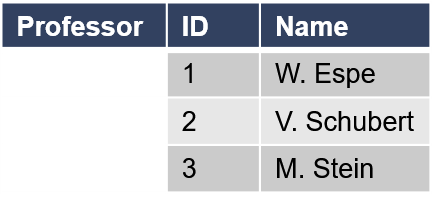
\includegraphics[scale=0.5]{img/ERM-BeispielEntitaetsmengeProfessor.png}
		\end{minipage}
	  \quad Entit\"atsmenge f\"ur \emph{Professor}
	\end{figure}    
	\begin{figure}
  	Entit\"atstyp \emph{Fach} $\Rightarrow$\quad 
	  \begin{minipage}{0.3\linewidth}
		 \centering
		 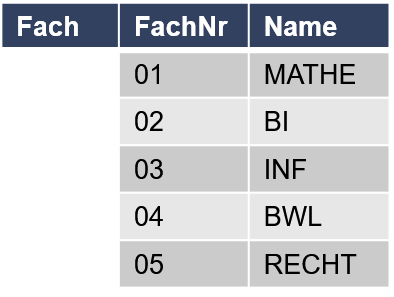
\includegraphics[scale=0.5]{img/ERM-BeispielEntitaetsmengeFach.png}
	  \end{minipage}
	  \quad Entit\"atsmenge f\"ur \emph{Fach}
  \end{figure}    
\end{frame}

\begin{frame}{\insertsection}
\framesubtitle{Mengentheoretische Sicht}
\structure{Beziehungstyp $\equiv$ Relation zwischen Entit\"atsmengen (mit Semantik angereichert)}
	\begin{figure}
		Beziehungstyp \emph{Lehre} $\Rightarrow$
		\begin{minipage}{0.4\linewidth}    	
 	    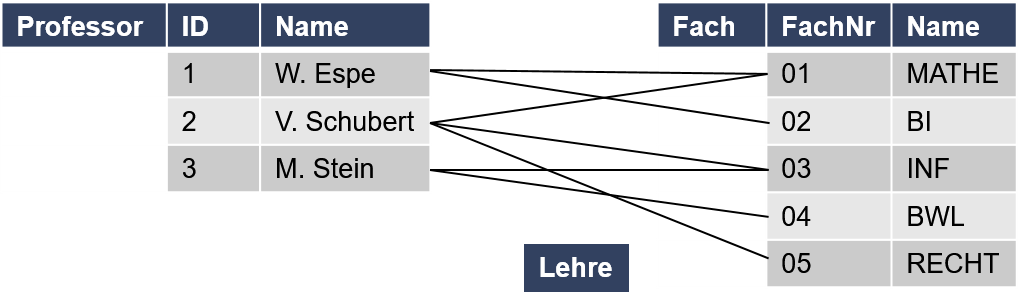
\includegraphics[scale=0.35]{img/ERM-BeispielRelationLehreProfessorFach.png}
 	  \end{minipage} 
    \quad Relation f\"ur \emph{Lehre}
 	\end{figure}    
\end{frame}

\begin{frame}{\insertsection}
\framesubtitle{Mengentheoretische Sicht -- Wiederholung Mengenlehre}
\begin{itemize}
 \item Eine (endliche) \emph{Menge} $M$ besteht aus \emph{Elementen} $e_1$, $e_2$, $\ldots$, $e_m$
   \begin{itemize}
	   \item Bezeichnung: $M=\{e_1, e_2,\ldots , e_m\}$
	 \end{itemize}
 \item Jedes Element $e_i$ f\"ur $i= 1, 2,\ldots,m$ geh\"ort zu der Menge $M$
   \begin{itemize}
   	\item Bezeichnung: $e_i\in M$
   \end{itemize}
 \item Die \emph{M\"achtigkeit} $\vert M\vert$ einer (endlichen) Menge $M$ ist die Anzahl der Elemente von $M$.
\end{itemize}
\onslide\pause 
\abs\abs
\structure{\textbf{Wichtige Eigenschaften von Mengen:}}
\begin{itemize}
	\item In einer Menge existieren keine doppelten Elemente
	\item Die Elemente einer Menge sind nicht geordnet
\end{itemize}
\end{frame}

\begin{frame}{\insertsection}
\framesubtitle{Mengentheoretische Sicht -- Wiederholung Mengenlehre}
\begin{itemize}
	\onslide 
	\item Ein Element $e$ kann zu zwei Mengen $M_1$ und $M_2$ geh\"oren: $e\in M_1$ und $e\in M_2$\\[4pt]	
	\pause 
	\item Die Menge aller Elemente, die zu $M_1$ und $M_2$ geh\"oren bilden wieder eine Menge, die sogenannte \emph{Schnittmenge} 
	$M_1\cap M_2$
	\begin{equation*}
	M_1\cap M_2=\{ e\mid e\in M_1\text{ und } e\in M_2\}
	\end{equation*}
	\pause
	\item Die Menge aller Elemente, die zu $M_1$ oder zu $M_2$ geh\"oren bilden wieder eine Menge, die sogenannte \emph{Vereinigungsmenge}
	$M_1\cup M_2$
	\begin{equation*}
	M_1\cup M_2=\{ e\mid e\in M_1\text{ oder } e\in M_2\}
	\end{equation*}
\end{itemize}
\end{frame}

\begin{frame}{\insertsection}
\framesubtitle{Mengentheoretische Sicht -- Wiederholung Mengenlehre}
\begin{itemize}
\onslide 
\item Ist $M$ eine Menge, deren Elemente zu $N$ geh\"oren, dann hei\ss t $M$ \emph{Untermenge} von $N$.\\[4pt]
Bezeichnung: $M\subseteq N$\\[8pt]
\pause
\item Gilt $M\subseteq N$ und $N\subseteq M$, dann folgt daraus $M=N$.\\[8pt]
\pause
\item
Die Menge aller Elemente von $M_2$, die nicht zu der Menge $M_1$ geh\"oren, hei\ss t die Differenz von $M_2$ und $M_1$.\\[4pt]
Bezeichnung: $M_2 - M_1$\\[8pt]
\pause
\item Es gilt: $M\cap N = M - (M - N) = N- (N - M)$ (\"Ubungsaufgabe!)
\end{itemize}
\end{frame}

\begin{frame}{\insertsection}
\framesubtitle{Mengentheoretische Sicht -- Wiederholung Mengenlehre}
\begin{definition}[Funktion]
\begin{enumerate}
	\item 
	Seien $M_1$ und $M_2$ zwei Mengen. Eine Funktion $f:M_1\to M_2$ ist eine eindeutige Zuordnung von Elementen 
	aus $M_1$ auf Elemente aus $M_2$. Das hei\ss t, jedem $x\in M_1$ wird genau ein $y\in M_2$ zugeordnet. 
	\\[4pt]
	Bezeichnung: $x\overset{f}{\mapsto} y$ oder $y=f(x)$.
	\\[4pt]
	\item Zwei Funktionen $f,g:M_1\to M_2$ sind gleich, falls $f(x)=g(x)$ f\"ur jedes $x\in M_1$ gilt. 
	\\[4pt]
	Bezeichnung: $f=g$.
\end{enumerate}
\end{definition}
\end{frame}

\begin{frame}{\insertsection}
\framesubtitle{Mengentheoretische Sicht -- Wiederholung Mengenlehre}
\begin{itemize}
	\onslide
	\item Für zwei (endliche) Mengen $M_1=\{e_1, e_2,\ldots , e_n\}$ und $M_2=\{c_1, c_2, \ldots , c_m\}$ kann man das \emph{kartesische Produkt} 
	$M_1\times M_2$ bilden:
	\begin{itemize} 
		\item Das kartesische Produkt $M_1\times M_2$ ist die Menge aller Tupel $(e_i,c_j)$ mit $e_i\in M_1$ und $c_j\in M_2$.
		\item Das hei\ss t
		\begin{equation*}
		M_1\times M_2=\{(e_1,c_1), (e_1,c_2),\ldots, (e_1,c_m),(e_2,c_1), \ldots, (e_n,c_m)\}
		\end{equation*}
	\end{itemize}
  \pause
	\item Entsprechend kann man aus $r$ (endlichen) Mengen $M_1$, $M_2$, $\ldots$, $M_r$ das $r$-fache kartesische Produkt 
	$M_1\times M_2 \times \cdots \times M_r$ aller $r$-Tupel bilden:
	\begin{equation*}
	\begin{split}
	M_1\times M_2 \times \cdots \times M_r &=\{(e_1,c_1, \ldots, x_1), (e_1,c_1,\ldots, x_2),\ldots, (e_n,c_m, \ldots, x_p)\}\\
	&=\{\underbrace{(e,c,\ldots,x)}_\text{r-Tupel} \mid e\in M_1, c\in M_2,\ldots ,x\in M_r\}
	\end{split} 
	\end{equation*} 
\end{itemize}
\end{frame}

\begin{frame}{\insertsection}
\framesubtitle{Mengentheoretische Sicht -- Relationen}
\begin{definition}[Zweistellige Relationen]
	Seien $M_1$ und $M_2$ Mengen. Eine zweistellige Relation $R$ ist eine Teilmenge des kartesischen Produktes $M_1\times M_2$.
\begin{equation*} 
R \subseteq M_1 \times M_2
\end{equation*} 
\end{definition}
\abs 
Es gilt: $\vert M_1\times M_2\vert = \vert M_1\vert\cdot \vert M_2\vert$
\abs\abs
\alert{Beispiele!}
\end{frame}

\begin{frame}{\insertsection}
\framesubtitle{Mengentheoretische Sicht -- Relationen}
\begin{definition}[r-stellige Relationen]
Seien $M_1$, $M_2$, $\ldots$, $M_r$ Mengen. Eine $r$-stellige Relation $R$ ist eine Teilmenge des $r$-fachen 
kartesischen Produktes $M_1 \times M_2 \times \cdots \times M_r$.
\begin{equation*} 
R \subseteq M_1 \times M_2 \times \cdots \times M_r
\end{equation*} 
\end{definition}
\abs 
Es gilt: $\vert M_1\times \ldots \times M_r\vert = \vert M_1\vert\cdot\ldots\cdot \vert M_r\vert =\prod_{i=1}^r\vert M_i\vert$
\abs\abs
\alert{Beispiele!}
\end{frame}

\begin{frame}{\insertsection}
\framesubtitle{Mengentheoretische Sicht -- Zur"uck zum Beispiel}
\centering 
\begin{minipage}[c]{0.3\linewidth}
	\begin{figure} 
		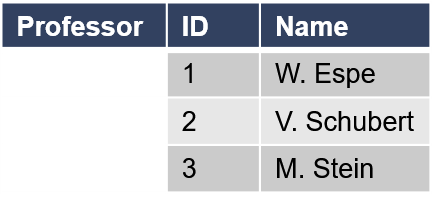
\includegraphics[scale=0.45]{img/ERM-BeispielEntitaetsmengeProfessor.png}
	\end{figure}
\end{minipage}
\begin{minipage}[c]{0.5\linewidth}
	\begin{equation*}
	\begin{split} 
	&\text{Entit\"atsmenge f\"ur \emph{Professor}}\\
	&=\{e_{P(1, \text{Espe})},e_{P(2,\text{Schubert})},e_{P(3, \text{Stein})}\}
	\end{split}
	\end{equation*}
\end{minipage}
\abs\abs\abs 
\begin{minipage}[c]{0.3\linewidth}
	\begin{figure} 
		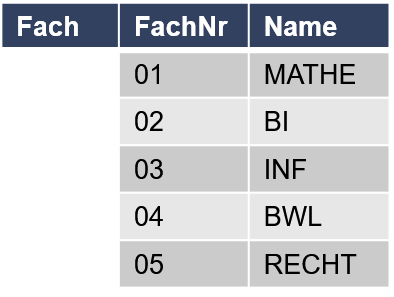
\includegraphics[scale=0.45]{img/ERM-BeispielEntitaetsmengeFach.png}
	\end{figure}
\end{minipage}
\begin{minipage}[c]{0.5\linewidth}
	\begin{equation*}
	\begin{split} 
	&\text{Entit\"atsmenge f\"ur \emph{Fach}}\\
	&=\{e_{F(01,\text{MATHE})},e_{F(02,\text{BI})},\\
	&\quad\,\,\,\, e_{F(03,\text{INF})},e_{F(04,\text{BWL})},e_{F(05,\text{RECHT})}\}
	\end{split}
	\end{equation*}
\end{minipage}
\end{frame} 

\begin{frame}{\insertsection}
\framesubtitle{Mengentheoretische Sicht -- Zur"uck zum Beispiel}
\centering 
\begin{minipage}[c]{0.5\linewidth}
\begin{figure} 
	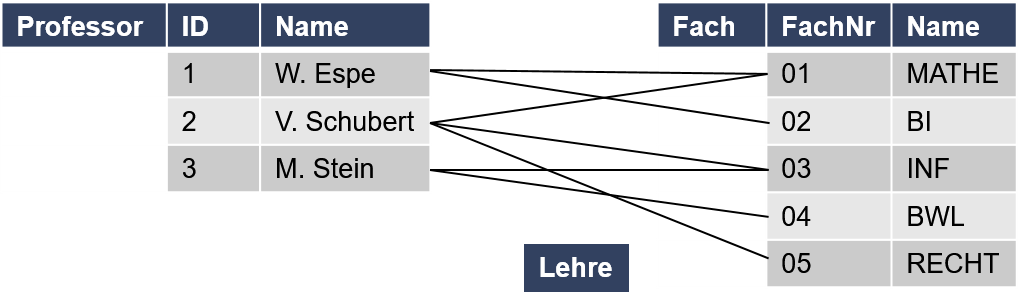
\includegraphics[scale=0.45]{img/ERM-BeispielRelationLehreProfessorFach.png}
\end{figure}
\end{minipage}
\abs 
\begin{minipage}[c]{0.5\linewidth}
\begin{equation*}
\begin{split} 
&\text{Relation f\"ur \emph{Lehre}}\\
&=\{(e_{P(1, \text{Espe})}, e_{F(01,\text{MATHE})}),(e_{P(1, \text{Espe})}, e_{F(02,\text{BI})}),\\
&\quad\,\,\,\,(e_{P(2,\text{Schubert})}, e_{F(01,\text{MATHE})}),(e_{P(2,\text{Schubert})}, e_{F(03,\text{INF})}),\\
&\quad\,\,\,\,(e_{P(2,\text{Schubert})}, e_{F(05,\text{RECHT})}),(e_{P(3, \text{Stein})}, e_{F(03,\text{INF})}),\\
&\quad\,\,\,\,(e_{P(3, \text{Stein})}, e_{F(04,\text{BWL})})\}
\end{split}
\end{equation*}
\end{minipage}
\end{frame} 

\begin{frame}{\insertsection}
\framesubtitle{Mengentheoretische Sicht}
\begin{itemize}
	\item Seien $E_1$, $E_2$, $\ldots$, $E_r$ Entit\"atstypen und $\mathcal{M}(E_1)$, $\mathcal{M}(E_2)$, $\ldots$, $\mathcal{M}(E_r)$ 
	die zugeh\"origen Entit\"atsmengen.
	\item Sei $B$ der Beziehungstyp zwischen den Entit\"aten $E_1$, $E_2$, $\ldots$, $E_r$. 
	Dann bezeichnet $\mathcal{R}(B)$ die zugeh\"orige Relation. 
	\begin{equation*} 
	\mathcal{R}(B)\subseteq	\mathcal{M}(E_1)\times\mathcal{M}(E_2)\times\cdots\times\mathcal{M}(E_r)
	\end{equation*} 
\end{itemize}
\end{frame} 

\begin{frame}{\insertsection}
%\framesubtitle{\insertsubsection}
\structure{Graphische Notation}
\newline
\begin{itemize}
	\item Entit\"atstypen: Rechtecke mit Namen des Entit\"atstyps
		\begin{figure}
			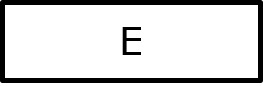
\includegraphics[scale=0.5]{img/ERM-EntitaetTyp.png}
		\end{figure}
	\item Beziehungstypen: Rauten mit Namen des Beziehungstyps
		\begin{figure}
			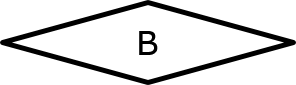
\includegraphics[scale=0.5]{img/ERM-BeziehungTyp.png}
		\end{figure}
	\item Attribute: Ovale mit Namen des Attributs
	  \begin{figure}
	  	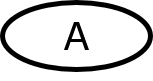
\includegraphics[scale=0.5]{img/ERM-AttributTyp.png}
  	\end{figure}
\end{itemize}
\end{frame}

\begin{frame}{\insertsection}
%\framesubtitle{\insertsubsection}
\structure{Graphische Notation}
\begin{itemize}
	\item Entit\"atstypen durch Linien mit Beziehungstypen verbunden
	\begin{figure}
		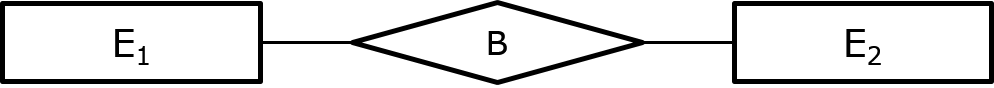
\includegraphics[scale=0.5]{img/ERM-EntitaetRelationTyp.png}
	\end{figure}  
	\item Entit\"ats- und Beziehungstypen durch Linien mit Attributen verbunden
	\begin{figure}
	 \centering
	 \begin{minipage}{0.3\linewidth}
		\centering
		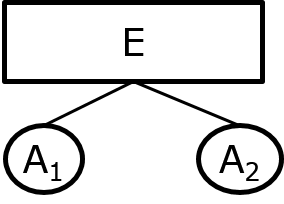
\includegraphics[scale=0.5]{img/ERM-EntitaetAttributTyp.png}
	 \end{minipage}
 	 \begin{minipage}{0.3\linewidth}
		\centering
		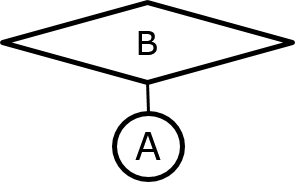
\includegraphics[scale=0.5]{img/ERM-RelationAttributTyp.png}
   \end{minipage}
	\end{figure}    
\end{itemize}
\end{frame}

\begin{frame}{\insertsection}
%\framesubtitle{\insertsubsection}
\structure{Graphische Notation -- Beispiel}
\begin{itemize}
	\item Entit\"atstypen
 	 \begin{figure}
		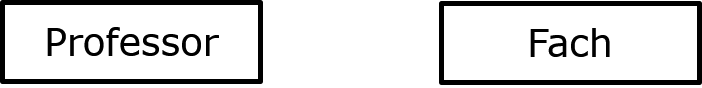
\includegraphics[scale=0.5]{img/ERM-BeispielEntitaetTyp.png}
	 \end{figure}  
	\item Beziehung der beiden Entit\"atstypen
	 \begin{figure}
	  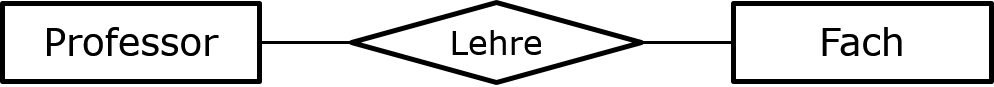
\includegraphics[scale=0.5]{img/ERM-BeispielEntitaetRelationTyp.png}
   \end{figure}  
 \item ... attributiert
  \begin{figure}
	 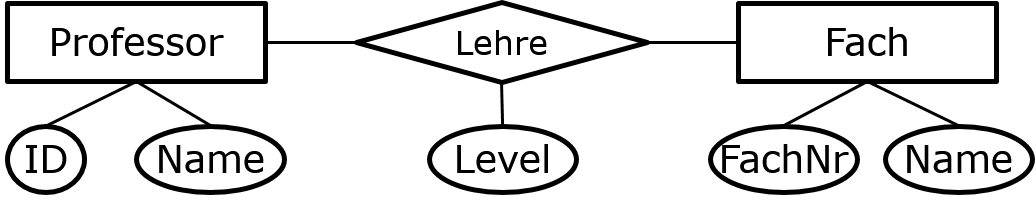
\includegraphics[scale=0.5]{img/ERM-BeispielEntitaetRelationAttributTyp.png}
  \end{figure}  
\end{itemize}
\end{frame}

\begin{frame}{\insertsection}
\framesubtitle{Noch ein Beispiel}
\begin{columns}
	\begin{column}{.31\textwidth}
		\begin{figure}
			\begin{tikzpicture}[node distance=7em]
			\node[entity] (Kunde) {\small Kunde}; 
			\node[attribute] (knr) [above left of=Kunde] {{\small KNR}} edge (Kunde); 
			\node[attribute] (name) [above of=Kunde] {\small Name} edge (Kunde); 
			\end{tikzpicture}
			\caption{Entit\"atstyp}
		\end{figure}		
	\end{column}
	
	\begin{column}{.31\textwidth}
		\begin{figure}
			\begin{tabbing}
				\textbf{Kunde} \= Name \= \kill
				\textbf{Kunde:}\\
				KNR \> 1 \\
				Name \> Mustermann \\
			\end{tabbing}
			\caption{Entit\"at}
		\end{figure} 
	\end{column}
	
	\begin{column}{.31\textwidth}
		\begin{figure}
			\begin{tabular}{|c|c|}\hline
				\multicolumn{2}{|c|}{\small \textbf{Kunde}}\\\hline\hline
				\small \textbf{KNR} & \small \textbf{Name} \\\hline 
				\small 1 &\small Mustermann \\\hline 
				\small 2 & \small Musterfrau \\\hline 
				$\cdots$ & $\cdots$ \\\hline
			\end{tabular}				
			\caption{Entit\"atsmenge}
		\end{figure} 
	\end{column}
\end{columns}
% \alert{Wertebereiche / Domänen werden in ER-Diagrammen nicht festgehalten!}
\end{frame}

\begin{frame}{\insertsection}
\framesubtitle{Grad einer Beziehung}
\begin{definition}[Grad von Beziehungen]
	\label{def:gradVonBeziehungen}
	Der \textit{Grad} einer Beziehung ist die Anzahl der an der Beziehung teilnehmenden Entit\"atstypen.
\end{definition}
\begin{itemize}
	\item Beziehungen vom Grad 2 bezeichnet man als \textit{binäre} Beziehungen
	\item Beziehungen vom Grad 3 bezeichnet man als \textit{ternäre} Beziehungen
	\item Beziehungen vom Grad n bezeichnet man als $n$\textit{-äre} Beziehungen
\end{itemize}
\end{frame}

\begin{frame}[t]{\insertsection}
\framesubtitle{Rekursive Beziehungen}
\begin{itemize}
\item Rekursive Beziehungen sind erlaubt
\item Jeder Entitätstyp, der an einer Beziehung teilnimmt, spielt eine bestimmte Rolle.
\end{itemize}
\begin{figure}
	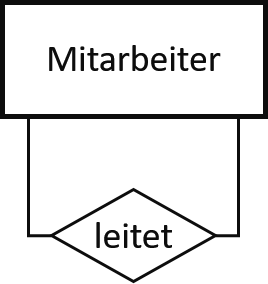
\includegraphics[scale=0.5]{img/ERM-Rekursiv.png}	
%  \begin{tikzpicture}[node distance=2em]
%   \node[entity] (ma) {\small Mitarbeiter}; 
%   \node[relationship] (leitet) [below=of ma] {\small{leitet}}; 
%   \draw (ma.west) |- (leitet.west) node[midway,above,rotate=90, xshift=10mm] {\tiny Vorgesetzter}; 
%   \draw (ma.east) |- (leitet.east) node[midway,below,rotate=90, xshift=10mm] {\tiny Angestellter};  			
%   \end{tikzpicture}
   \caption{Rekursive Beziehung}
\end{figure}		
\end{frame}

\begin{frame}[t]{\insertsection}
\framesubtitle{Attributarten}
\structure{Mehrere Attributtypen kommen in ER-Diagrammen vor:}
\onslide
\begin{itemize}
	\item Atomare Attribute, die nicht geteilt werden können (z.B. Alter, Postleitzahl, Nachname)
	\item Zusammengesetzte Attribute (z.B. das Attribut \textit{Anschrift}, welches aus weiteren Attributen
	PLZ, Ort und Straße zusammengesetzt ist)
	\pause
	\item Einwertige Attribute, bei denen zu einem bestimmten Zeitpunkt \textit{genau ein Wert} existiert 
	\item Mehrwertige Attribute, bei denen zu einem bestimmten Zeitpunkt mehrere Werte existieren können (z.B. wenn eine Person zwei akademische Titel hat)
	\pause
	\item Abgeleitete Attribute, deren Wert sich aus anderen Attributen herleiten lässt (z.B. kann ein Attribut \textit{Alter} aus dem Geburtsdatum errechnet werden)
\end{itemize}
\pause
\abs
\structure{\texttt{null}-Eigenschaft:}
\begin{itemize}
	\item \texttt{null}-Attribute sind Attribute, die f\"ur manche Entitäten nicht belegt sind. 
	\begin{itemize}
		\item \alert{Achtung: \texttt{null}-Attribute bergen Interpretationsspielraum!} 
	\end{itemize}
\end{itemize}
\end{frame}

\begin{frame}{\insertsection}
\framesubtitle{Attributtypen -- Graphische Notation}
\begin{figure}
\begin{tikzpicture}[node distance=7em]
\node[attribute] (einfach) {\small Einfach}; 
\node[derived attribute] (abgeleitet) [right=of einfach] {\small Abgeleitet} ; 
\node[multi attribute] (multi) [right=of abgeleitet] {\small Mehrwertig} ;
\node[attribute, align=center] (zusammen) [below=0.5cm of abgeleitet] {\small Zusammengesetzt\\Ort};
\node[attribute] (plz) [below left=3em of zusammen] {\small PLZ} edge (zusammen); 
\node[attribute] (str) [below right=3em of zusammen] {\small Str} edge (zusammen); 
\end{tikzpicture}
\caption{Attributtypen}
\end{figure}		
\end{frame}

\begin{frame}[t]{\insertsection}
\framesubtitle{Identifizierbarkeit von Entitäten}
\begin{definition}[Schlüssel]
Ein Schlüssel ist ein Attribut oder eine Attributkombination, mit dem eine Entität eines Entitätstyps eindeutig identifiziert 
werden kann.\label{def:er:key}
\end{definition}
\onslide\pause
\abs
Ein Schlüsselattribut wird durch Unterstreichung gekennzeichnet. Falls notwendig kann ein 
künstliches Schlüsselattribut (Surrogatschlüssel) zugefügt werden.
\begin{figure}
\begin{tikzpicture}[node distance=1em]
\node[entity] (Kunde) {\small Kunde}; 
\node[attribute] (knr) [above left=1em of Kunde] {\key{\small KNR}} edge (Kunde); 
\node[attribute] (name) [above right=1em of Kunde] {\small Name} edge (Kunde); 
\end{tikzpicture}
\caption{Entitätstyp mit Schlüsselattribut KNR}
\end{figure}		
\end{frame}

%\begin{frame}[t]{\insertsection}
%\framesubtitle{Noch ein Beispiel}
%\begin{figure}
%	\begin{tikzpicture}[node distance=2em]
%	\node[entity] (Student) {\small Student}; 
%	\node[attribute] (knr) [above left=2em of Student] {\key{\small MNR}} edge (Student); 
%	\node[attribute] (name) [above=2em of Student] {\small Name} edge (Student);
%	\node[relationship] (betreut) [right=of Student] {\small{betreut}} edge (Student); 
%	\node[entity] (prof) [right=of betreut]  {\small{Professor}} edge (betreut);
%	\node[attribute] (profnr) [above=of prof] {\small{\key{ProfNr}}} edge (prof);
%	\node[attribute] (profname) [above right=of prof] {\small{Name}} edge (prof);
%	\end{tikzpicture}
%	%	\caption{Beziehungstyp zwischen Entitätstypen}
%\end{figure}		
%\abs\alert{Achtung: Es gibt keine explizit vorgegebene Leserichtung!}
%\end{frame}

\begin{frame}[t]{\insertsection}
\framesubtitle{Noch ein Beispiel}
Abbildung \ref{er:attrel} drückt das Schreiben von Klausuren an einem bestimmten Datum aus.
\begin{figure}
	\begin{tikzpicture}[node distance=2em]
	\node[entity] (Student) {\small Student}; 
	\node[attribute] (knr) [above left=2em of Student] {\key{\small MNR}} edge (Student); 
	\node[attribute] (name) [above=2em of Student] {\small Name} edge (Student);
	\node[relationship] (schreibt) [right=of Student] {\small{schreibt}} edge node[auto,swap] {} (Student); 
	\node[entity] (klausur) [right=of schreibt]  {\small{Klausur}} edge node[auto,swap] {} (schreibt); 
	\node[attribute] (datum)[above=of schreibt] {\small{Datum}} edge (schreibt); 
	\node[attribute] (knr) [above=of klausur] {\small{\key{KNr}}} edge (klausur);
	\node[attribute] (kname) [above right=of klausur] {\small{Fach}} edge (klausur);
	\end{tikzpicture}
	\caption{\label{er:attrel}ER-Diagramm mit attributierter Beziehung}
\end{figure}		
\alert{Zu beachten: Es gibt keine explizit vorgegebene Leserichtung! Das ist implizite Semantik.}
\end{frame}

\begin{frame}{\insertsection}
\framesubtitle{Kardinalit\"aten -- Motivation}
\begin{itemize}
	\item Eine Person kann \textbf{keines}, \textbf{eines} oder \textbf{mehrere} \underline{Autos} besitzen
	\item Eine Person ist mit \textbf{keiner} oder \textbf{einer} \underline{Person} verheiratet
  \item Eine Person besitzt \textbf{einen} \underline{Ausweis}
	\item Ein Professor an einer Fakult\"at liest \textbf{keine}, \textbf{eine} oder \textbf{mehrere} \underline{Vorlesungen}
	\item Eine Vorlesung in einer Fakult\"at wird von \textbf{einem} oder \textbf{mehreren} \underline{Professoren} gelesen	
\end{itemize}
\end{frame}

%
% Chen-UML-Notation
%
\begin{frame}{\insertsection}
\framesubtitle{Kardinalit\"aten}
\begin{definition}[look-across-Kardinalit\"at]\label{carddef}
	Seien $E_1$, $E_2$, $\ldots$, $E_n$ Entit\"atstypen und $B$ ein Beziehungstyp zwischen diesen 
	Entit\"aten. 
	\abs
	Die Kardinalit\"at $C_i$ des Entit\"atstyps $E_i$ ($i\in\{1,\ldots,n\}$) gibt an, mit wie vielen 
	Entit\"aten des Typs $E_i$ ein vorgegebenes Tupel $(e_1,\ldots,e_{i-1},e_{i+1},\ldots,e_n)$ 	
	aus Entit\"aten der anderen Entit\"atstypen in Beziehung stehen kann.
\end{definition}
\abs\onslide\pause 
Es gibt unter anderem die Kardinalit\"aten $'1'$, $'n'$, $'0..1'$, $'0..n'$:
\begin{description}[leftmargin=0cm]
	\item[$1$:] Mit genau einer Entit\"at steht das vorgegebene Tupel in Beziehung.
	\item[$n$:] Mit einer oder mehreren Entit\"aten steht das vorgegebene Tupel in Beziehung.
	\item[$0..1$:] Mit keiner oder einer Entit\"at steht das vorgegebene Tupel in Beziehung.
	\item[$0..n$:] Mit keiner, einer oder mehreren Entit\"aten steht das vorgegebene Tupel in Beziehung.
\end{description}
\end{frame}

\begin{frame}{\insertsection}
\framesubtitle{Kardinalit\"aten -- Graphische Notation}
\begin{itemize}
	\item Kardinalit\"at $C_i$ von Entit\"atstyp $E_i$ in Beziehung $B$
\end{itemize}
\begin{figure}
	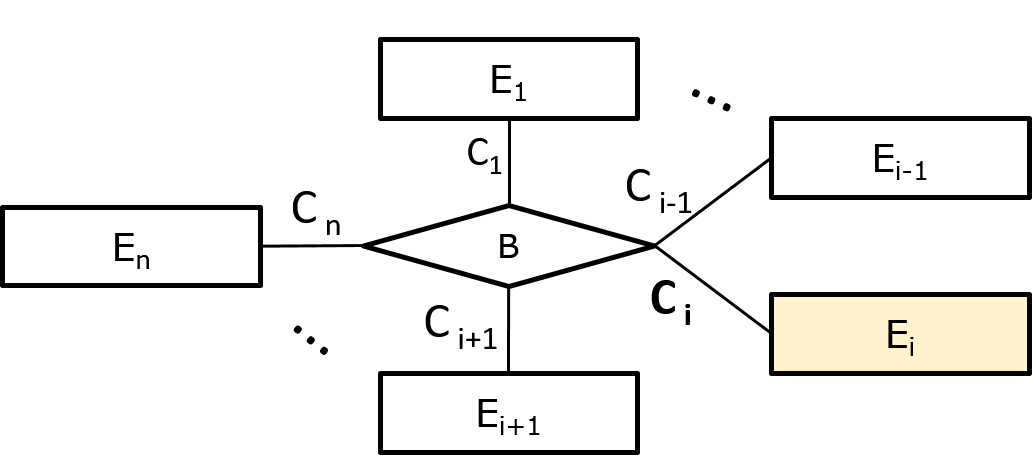
\includegraphics[scale=0.5]{img/ERM-Kardinalitaet.png}
\end{figure}  
% \alert{Machen Sie sich die Definition \ref{carddef} anhand von Beispielen klar.}
\end{frame}

\begin{frame}{\insertsection}
\framesubtitle{Kardinalit\"aten}
\begin{block}{Kardinalit\"aten anhand von Beispielen}
	\begin{description}[leftmargin=0cm]
		\item[1:n] Eine Person besitzt eines oder mehrere Autos. Jedes Auto wird von genau  
		einer Person besessen. Zwischen den Entit\"atstypen Person und Auto besteht ein [1:n]-Beziehungstyp.
		\item[n:m] Eine Person arbeitet an einem oder mehreren Projekten. Jedes Projekt wird durch 
		eine oder mehrere Personen bearbeitet.
		\item[1:1] Eine Person besitzt genau einen Ausweis und ein Ausweis geh\"ort zu genau einer Person. 
		\item[0..n\,:\,1] Ein Mitarbeiter besitzt genau einen Angestelltenstatus. Ein Angestelltenstatus geh\"ort zu keinem, einem 
		oder mehreren Mitarbeitern.
	\end{description}
\end{block}
 \alert{Zeichnen Sie die entsprechenden ERM-Diagramme.}
\end{frame}

\begin{frame}[t]{\insertsection}
\framesubtitle{Kardinalitäten}
\begin{figure}
	\begin{tikzpicture}[node distance=2em]
	\node[entity] (Student) {\small Student}; 
	\node[attribute] (knr) [above left=2em of Student] {\key{\small MNR}} edge (Student); 
	\node[attribute] (name) [above=2em of Student] {\small Name} edge (Student);
	\node[relationship] (betreut) [right=of Student] {\small{betreut}} edge node[auto,swap] {n} (Student); 
	\node[entity] (prof) [right=of betreut]  {\small{Professor}} edge node[auto,swap] {1} (betreut);
	\node[attribute] (profnr) [above=of prof] {\small{\key{ProfNr}}} edge (prof);
	\node[attribute] (profname) [above right=of prof] {\small{Fach}} edge (prof);
	\end{tikzpicture}
	\caption{ER-Diagramm mit Kardinalitäten}
\end{figure}		
 \alert{Was sagt dieses ERM-Diagramm aus?}
\end{frame}

\begin{frame}{\insertsection}
\framesubtitle{Kardinalitäten auf Entit\"atsmengen und Relationen}
\structure{[1:1]-Beziehung}
\newline 
(E) 1: Ordnet einer gegebenen Entit\"at $f_j \in F$ genau eine Entit\"at in $E$ zu. 
\newline 
(F) 1: Ordnet einer gegebenen Entit\"at $e_i \in E$ genau eine Entit\"at in $F$ zu. 
\begin{figure}
	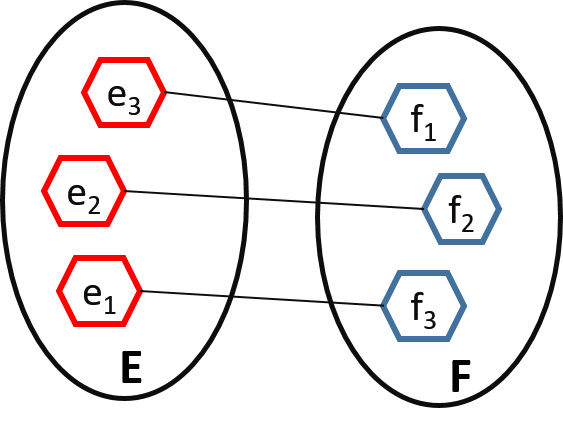
\includegraphics[scale=0.5]{img/ERM-11-11-Relation.png}
\end{figure}
\end{frame}

\begin{frame}{\insertsection}
\framesubtitle{Kardinalitäten auf Entit\"atsmengen und Relationen}
\structure{[n,m]-Beziehung}
\newline 
(E) n: Ordnet einer gegebenen Entit\"at $f_j \in F$ eine oder mehrere Entit\"aten in $E$ zu. 
\newline 
(F) m: Ordnet einer gegebenen Entit\"at $e_i \in E$ eine oder mehrere Entit\"aten in $F$ zu. 
\begin{figure}
	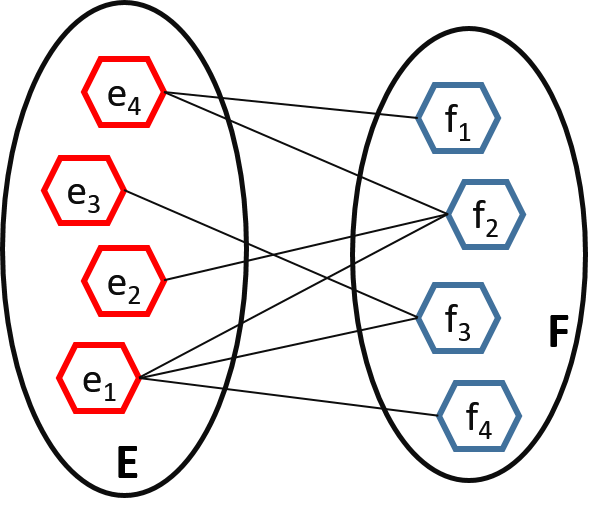
\includegraphics[scale=0.5]{img/ERM-1n-1m-Relation.png}
\end{figure}
\end{frame}

\begin{frame}{\insertsection}
\framesubtitle{Kardinalitäten auf Entit\"atsmengen und Relationen}
\structure{[0..1:0..1]-Beziehung}
  \newline 
  (E) 0..1: Ordnet einer gegebenen Entit\"at $f_j \in F$ keine oder eine Entit\"at in $E$ zu. 
\newline 
  (F) 0..1: Ordnet einer gegebenen Entit\"at $e_i \in E$ keine oder eine Entit\"at in $F$ zu. 
 \begin{figure}
	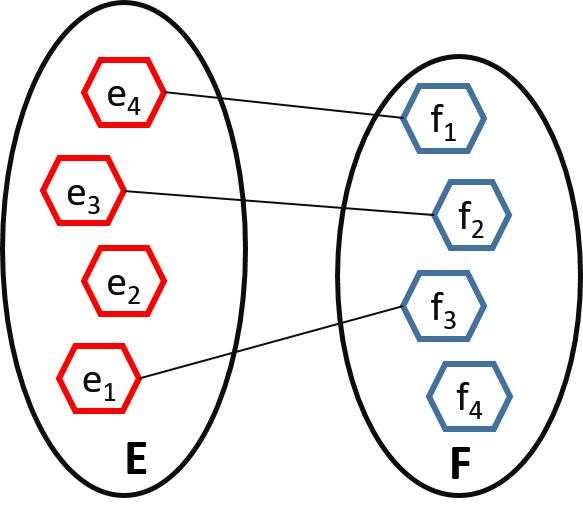
\includegraphics[scale=0.5]{img/ERM-1-1-Relation.png}
 \end{figure}
\end{frame}

\begin{frame}{\insertsection}
\framesubtitle{Kardinalitäten auf Entit\"atsmengen und Relationen}
\structure{[0..1:0..n]-Beziehung}
\newline 
(E) 0..1: Ordnet einer gegebenen Entit\"at $f_j \in F$ keine oder eine Entit\"at in $e_i\in E$ zu. 
\newline 
(F) 0..n: Ordnet einer gegebenen Entit\"at $e_i \in E$ keine, eine oder mehrere Entit\"aten in $F$ zu. 
\begin{figure}
	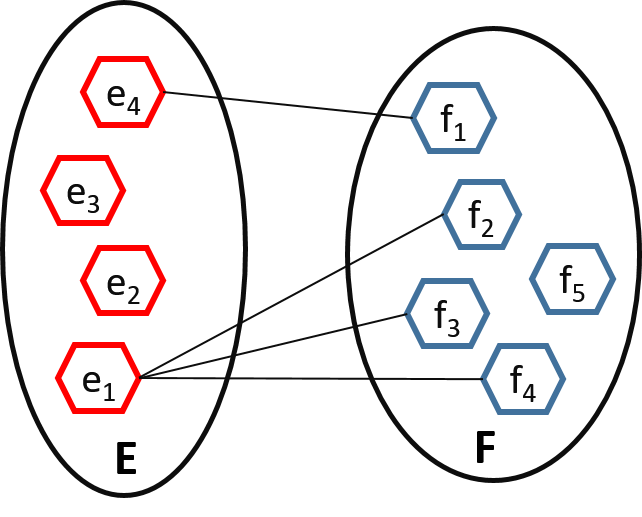
\includegraphics[scale=0.5]{img/ERM-1-n-Relation.png}
\end{figure}
\end{frame}

\begin{frame}{\insertsection}
\framesubtitle{Kardinalitäten auf Entit\"atsmengen und Relationen}
\structure{[0..n:0..m]-Beziehung}
\newline 
(E) 0..n: Ordnet einer gegebenen Entit\"at $f_j \in F$ keine, eine oder mehrere Entit\"aten in $E$ zu. 
\newline 
(F) 0..m: Ordnet einer gegebenen Entit\"at $e_i \in E$ keine, eine oder mehrere Entit\"aten in $F$ zu. 
\begin{figure}
	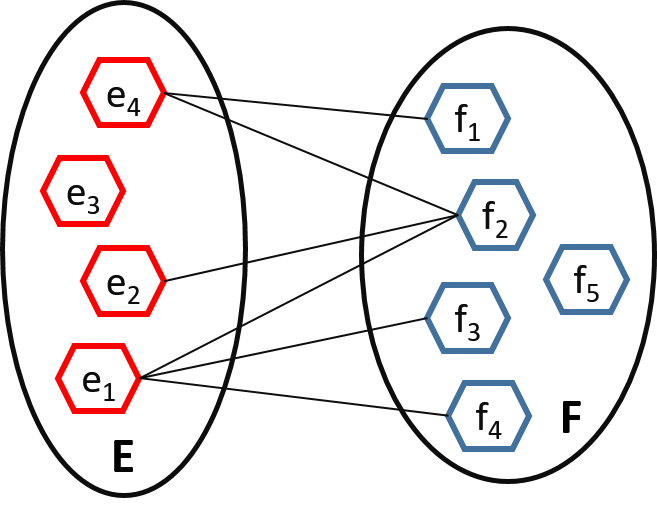
\includegraphics[scale=0.5]{img/ERM-n-m-Relation.png}
\end{figure}
\end{frame}

\begin{frame}{\insertsection}
\framesubtitle{Kardinalitäten auf Entit\"atsmengen und Relationen}
\structure{[n,0..m]-Beziehung}
\newline 
(E) n: Ordnet einer gegebenen Entit\"at $f_j \in F$ eine oder mehrere Entit\"aten in $E$ zu. 
\newline 
(F) 0..m: Ordnet einer gegebenen Entit\"at $e_i \in E$ keine, eine oder mehrere Entit\"aten in $F$ zu. 
\begin{figure}
	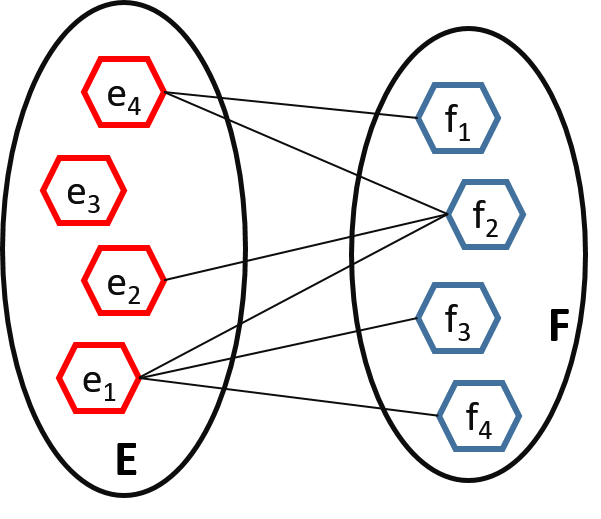
\includegraphics[scale=0.5]{img/ERM-1n-m-Relation.png}
\end{figure}
\end{frame}

\begin{frame}[t]{\insertsection}
\framesubtitle{Kardinalitäten -- tern\"are Beziehungen}
Beziehungen vom Grad $n>2$ benötigen eine besondere Beachtung! 
\abs
\structure{Beispiel:}
\begin{figure}	
	\begin{tikzpicture}[node distance=2em,scale=0.8, transform shape]
	\node[entity] (Professor) {\small Professor}; 
	\node[attribute] (pnr) [below left=of Professor] {\small{\key{PNr}}} edge (Professor);
	\node[relationship] (liest) [right=of Professor] {\small{betreut}} edge node[auto,swap] {1}  (Professor); 
	\node[entity] (Vorlesung) [right=of liest]  {\small{Student}} edge node[auto,swap] {n}  (liest);
	\node[attribute] (vnr) [below right=of Vorlesung] {\small{\key{SNR}}} edge (Vorlesung);
	\node[entity] (Raum) [below=of liest] {\small{Thema}} edge node[auto,swap] {1} (liest); 
	\node[attribute] (datum) [below right=of liest] {\small{{Note}}} edge (liest);
	\node[attribute] (rnr) [left=of Raum] {\small{\key{TNr}}} edge (Raum);
	\end{tikzpicture}	
	\caption{\label{er:ternary}ER-Diagramm mit tern\"arem Beziehungstyp}
\end{figure}		
\alert{\"Ubung: Welche Semantik hat dieses tern\"are Modell?}
\end{frame}

\begin{frame}{\insertsection}
\framesubtitle{Kardinalitäten -- $n$-\"are Beziehungen}
\begin{figure}
	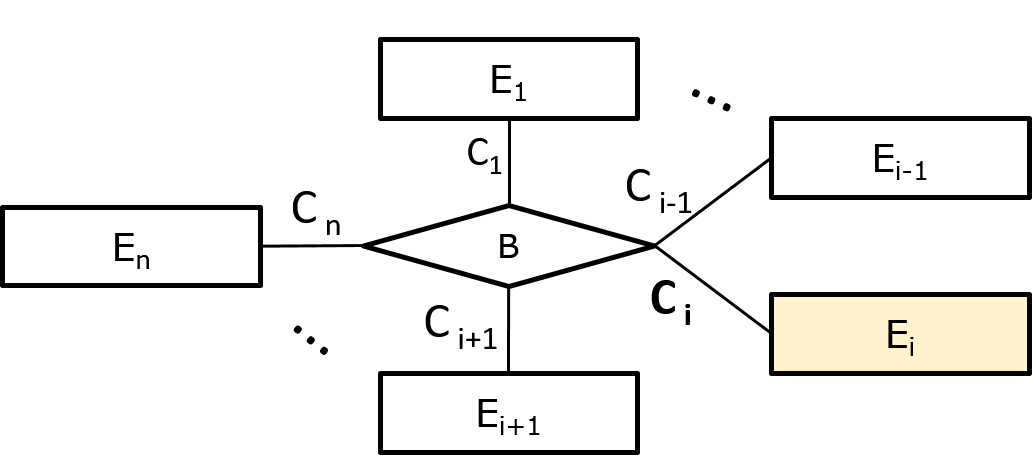
\includegraphics[scale=0.5]{img/ERM-Kardinalitaet.png}
\end{figure}  
\alert{\"Ubung: Machen Sie sich dieses allgemeine Diagramm anhand weiterer Beispiele klar.}
\end{frame}

\begin{frame}{\insertsection}
\framesubtitle{Totale Partizipation}
\begin{definition}[Totale Partizipation] Sei $B$ eine Beziehung zwischen den Entit\"atstypen $E_1, E_2,\ldots, E_n$. 
	Eine totale Partizipation des Entit\"atstyps $E_i$ in der Beziehung $B$ liegt vor, wenn es für \textbf{jede Entit\"at} $\mathbf{e_i}$
	vom Typ $E_i$ mindestens ein Tupel $(e_1,e_2,\ldots,\mathbf{e_i},\ldots,e_n)$ in der Relation $\mathcal{R}(B)$ gibt.
\end{definition} 
\abs
Totale Partizipation dr\"uckt also die zwingende Teilnahme aller Entit\"aten des Entitätstyps $E_i$ an der Beziehung aus. 
\end{frame}

\begin{frame}{\insertsection}
\framesubtitle{Totale Partizipation -- Graphische Notation}
\begin{figure}
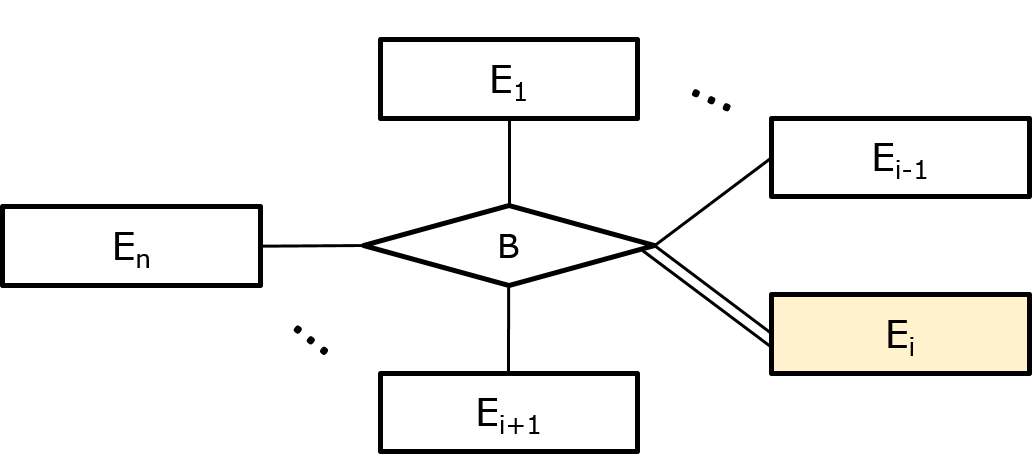
\includegraphics[scale=0.6]{img/ERM-TotalePartizipation.png}
\end{figure}  
\end{frame}

\begin{frame}{\insertsection}
\framesubtitle{Totale Partizipation -- Beispiel}
Abbildung \ref{er:total} dr\"uckt die totale Partizipation des Entit\"atstyps Professor an der Beziehung \emph{leitet} aus. 
Sie setzt also zwingend voraus, dass ein Professor auch (mindestens) einen Studiengang leitet.  
\begin{figure}
\begin{tikzpicture}[node distance=2em]
\node[entity] (Professor) {\small Studiengang}; 
\node[relationship] (leitet) [right=of Professor] {\small{leitet}} edge node[auto,swap] {} (Professor); 
\node[entity] (klausur) [right=of leitet]  {\small{Professor}} edge[total] node[auto,swap] {} (leitet);
\end{tikzpicture}
\caption{\label{er:total}ER-Diagramm mit totaler Partizipation}
\end{figure}		
\end{frame}

%@@@

\begin{frame}[label=isarelation]{\insertsection}
\framesubtitle{Spezielle Beziehungen}
\structure{Für die Abbildung von Generalisierungen / Vererbungen oder Aggregationen können spezielle Beziehungstypen eingesetzt werden.}

\begin{description}[leftmargin=0cm]
\item[is-a] Diese Beziehung verkörpert eine Generalisierung (z.B. Auto is-a Fahrzeug). Sie werden durch 
ein Dreieck dargestellt und verdienen besondere Beachtung bei der Überführung in ein Relationenschema (später in der Vorlesung).
\item[part-of] Diese Beziehung verkörpert eine Aggregation und wird mit einem normalen Beziehungssymbol versehen.
\end{description}

\begin{figure}
% 		\begin{tikzpicture}[node distance=2em]
% 			\node[entity] (Auto) {\small Auto}; 
% 			\node[isa] (ist) [right=of Auto] {\small{is a}} edge (Auto); 
% 			\node[entity] (fahrzeug) [right=of ist]  {\small{Fahrzeug}} edge  (ist);
% 			\node[relationship] (partof) x
% 		\end{tikzpicture}
% 		\caption{ER-Diagramm mit is-a Beziehung}
%	\end{figure}		
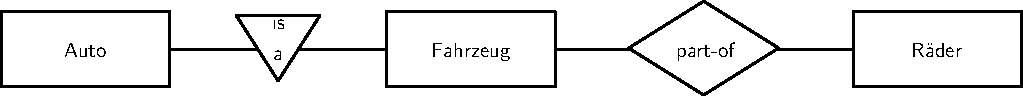
\includegraphics[scale=0.8]{img/genagg.pdf}
\caption{ER-Diagramm mit is-a Beziehung}
\end{figure}
\end{frame}

%\subsection{Schwache Entitäten}
\begin{frame}<1-2>[label=weakentity]
\frametitle<1-2>{\insertsection\framesubtitle{Schwache Entit\"aten}}
\frametitle<3>{\insertsection\framesubtitle{Schwache Entit\"aten -- Wiederholung Folie \ref{weakentity}}}
\onslide
{\structure{\textbf{Schwache Beziehungen}\\[4pt]}}
Beispiel: \emph{Raum} schwacher Entit\"atstyp, kann ohne \emph{Geb\"aude} nicht identifiziert werden.
\begin{figure}\scalebox{0.8}{
		\begin{tikzpicture}[node distance=2em]
		\node[entity] (geb) {\small Geb\"aude}; 
		\node[attribute] (gnr) [above left=2em of geb] {\key{\small GNR}} edge (geb); 
		\node[attribute] (ort) [above=2em of geb] {\small Name} edge (geb);
		\node[ident relationship] (besitzt) [right=of geb] {\small{besitzt}} edge node[auto,swap] {1} (geb); 
		\node[weak entity] (raum) [right=of besitzt]  {\small{Raum}} edge [total] node[auto,swap] {n} (besitzt); 
		\node[attribute] (rnr) [above=of raum] {\small{RNR}} edge (raum);
		\node[attribute] (profname) [above right=of raum] {\small{Groesse}} edge (raum);
		\end{tikzpicture}
	}
	\caption{\label{er:weak}Schwache Entität}
\end{figure}		
\pause[2]
\vspace{-1em}
\begin{itemize}
	\item Schwache Entit\"aten h\"angen in ihrer Existenz von Eigentümerentität ab.
	\item Identifikation schwacher Entitäten nur im Kontext der Eigent\"umerentit\"at.
	\item Eigent\"umerentit\"at kann keine, eine oder mehrere schwache Entit\"aten besitzen.
	\item Schwache Entit\"aten haben keine Attribute, die Schl\"ussel bilden k\"onnen.
\end{itemize}
\end{frame}

\begin{frame}[t]\frametitle{ER-Modellierung}
\framesubtitle{Entwurfsfragen}
\begin{itemize}
\item In ER-Diagrammen liegt der Fokus auf der Darstellung des Schemas, nicht der Instanzen
\item Die Namen von Entitätstypen, Beziehungstypen usw. sollten nach Möglichkeit die Semantik ausdrücken
\item Entitätstypen werden mit Substantiven im Singular benannt
\item ER-Diagramme werden meist stufenweise verfeinert: 
\begin{itemize}
\item Erstes Konzept mit grundlegenden Entitätstypen und Attributen
\item Einfügen von Beziehungstypen und Kardinalitäten
\item Attribute, die in mehreren Entitätstypen vorkommen, können auf einen eigenen Entitätstyp verfeinert werden
\item Zusammenlegung von Entitätstypen (z.B. Entitätstypen mit nur einem Attribut)
\end{itemize}
\end{itemize}
\end{frame}

\begin{frame}[t]\frametitle{ER-Modellierung}
\framesubtitle{Notationen}
\structure{Es existieren viele unterschiedliche Notationsformen von ER-Modellen:}
\begin{itemize}
\item Chen-Notation (nach Peter Chen, 1976)
\item UML-Notation
\begin{itemize}
\item Aussehen ähnlich wie Klassendiagramme 
\item Vererbung etc. möglich
\item Keine Beziehungen vom Grad $n>2$ erlaubt
\end{itemize}
\item Crow's Feet Notation 
\begin{itemize}
\item Ähnlich wie UML-Notation
\item Stellt Kardinalitäten durch Krähenfüsse dar
\end{itemize}
\end{itemize}
\abs
\structure{In der Vorlesung wird die (erweiterte) Chen-Notation weiter verwendet.}
\end{frame}

\section*{Übungsaufgaben}
\begin{frame}[t]
\frametitle{\insertsection}
\begin{alertblock}{Anwendungsfall: ToDo-Liste}
Modellieren Sie das Datenmodell für eine mehrbenutzerfähige ToDo-Liste (Anmerkung: Die Benutzer sollen \textit{nicht} gemeinsam an Projekten arbeiten!). 

\begin{itemize}
\label{todolist}
\item Zu den verschiedenen Benutzern werden Vorname, Nachname, Login und Passwort gespeichert 
\item Jeder Benutzer kann Projekte anlegen, bestehend aus einem Projektnamen 
\item Jedem Projekt können Aufgaben zugeordnet werden. Die Aufgaben werden pro Projekt beginnend mit der Aufgabennummer 1 angelegt und besitzen neben der Aufgabennummer einen Titel und einen Fertigstellungsgrad (in Prozent)
\end{itemize}
\end{alertblock}
\end{frame}

\section*{Übungsaufgaben}
\begin{frame}[t]
\frametitle{\insertsection}
\begin{alertblock}{Anwendungsfall: Flugbuchungssystem}
Eine Airline möchte ein Flugbuchungssystem erstellen. Sie erhalten die folgenden Informationen: 
\begin{itemize}
\item Jedem Flug mit einer Flugnummer wird eine konkrete Maschine mit entsprechenden Abflug- und Ankunftszeiten hinterlegt 
\item Jeder Flug startet und endet an einem Zielflughafen
\item Jeder Flug wird mit einer Maschine geflogen 
\item Eine Maschine wird von einem bestimmten Hersteller gebaut, besitzt eine Bezeichnung und hat eine Kapazität von $n$ Sitzplätzen
\item Zu jedem Passagier werden Name, Vorname, Geburtsdatum und Ausweisnummer gespeichert
\end{itemize}
Modellieren Sie den vorgegebenen Ausschnitt aus der realen Welt mittels eines ER-Diagramms.
\end{alertblock}
\end{frame}

\section{Relationales Datenmodell}

\begin{frame}<1>[label=codd]{\insertsection}
	%\framesubtitle{\insertsubsection}
	\begin{columns}
		\begin{column}{.68\textwidth}
			\begin{block}{Dr. Frank Edgar Codd (1923-2003)}
				\begin{itemize}
					\item Arbeitete bei IBM Research im IBM Almaden Research Center, St. Jose.
					\item Entwickelte das relationale Datenmodell im Jahre 1970: \emph{A relational Model for large shared data banks}
					\item ACM Turing Award im Jahre 1981 für \emph{\glqq fundamental and continuing contributions to the theory 
						and practice of database systems\grqq}
				\end{itemize}
			\end{block}

		\end{column}
		\begin{column}{.30\textwidth}
		 	\begin{figure}
				\pgfuseimage{codd}
			\end{figure}
		\end{column}
	\end{columns}
\end{frame}

\begin{frame}<1>[label=tabledef]{\insertsection}
	\framesubtitle{Motivation}
	Grob gesagt, organisiert das relationale Datenmodell Daten in Form von Tabellen und Beziehungen zwischen Tabellen.\abs
	\begin{columns}
		\begin{column}{.40\textwidth}
			Eine Tabelle besteht aus
			\begin{itemize}
				\item eindeutigem Namen
				\item Attributen (Spalten) über Wertebereichen (Domänen) 
				\item Tupeln oder \emph{Datens\"atzen} (Zeilen)
			\end{itemize}
		\end{column}
		\begin{column}{.56\textwidth}
			\begin{tabular}{|c|c|c|c|c|}\hline
				\multicolumn{5}{|c|}{\small \textbf{Kunde}}\\\hline\hline
				 \small \textbf{KNR} & \small \textbf{Vorname} & \small \textbf{Name} & \small \textbf{PLZ} & \small \textbf{Ort} \\\hline
				\small 1 &\small Elsa &\small Musterfrau &\small 68165 &\small Mannheim \\\hline
				\small 2 & \small Max &\small  Mustermann & \small 57234 &\small Wilnsdorf \\\hline
				$\cdots$ & $\cdots$ & $\cdots$ & $\cdots$ & $\cdots$ \\\hline
			\end{tabular}
		\end{column}
	\end{columns}
\end{frame}

\subsection{Formale Definition}

\begin{frame}
\frametitle{\insertsection}
\framesubtitle{\insertsubsection \ -- Datenbankschema}
\onslide
\begin{itemize}
	\item In logischen Datenmodellen werden Daten durch \emph{Datenbankschemata} beschrieben.
	\pause
	\item Ein Datenbankschema berücksichtigt dabei folgende Aspekte der Daten:
	\begin{itemize} 
		\item Struktur und Datentypen
		\item Zul\"assige Wertebereiche 
		\item Beziehungen
		\item Abh\"angigkeiten
		\item Identifizierbarkeit und Eindeutigkeit
	\end{itemize}
	\pause
	\item Durch ein Datenbankschema werden somit Bedingungen an die Daten definiert. 
	\begin{itemize}
		\item Diese Bedingungen nennt man \emph{Integrit\"atsbedingungen}.
		\item Integrit\"atsbedingungen k\"onnen syntaktischer oder (meistens) semantischer Natur sein.
		\item Die \"Uberpr\"ufung der Integrit\"atsbedingungen erfolgt durch das Datenbanksystem.
	\end{itemize}
	\pause
	\item Im relationalen Modell werden Tabellen durch ein \emph{Relationenschema} definiert.
	\begin{itemize}
		\item Ein Relationenschema ist Teil des Datenbankschemas.
	\end{itemize}	
\end{itemize}
\end{frame}

\begin{frame}
\frametitle{\insertsection}
\framesubtitle{\insertsubsection}
\begin{block}{\textbf{Vorab: Wiederholung des Begriffs \emph{Relation}}}
Seien $M_1$, $M_2$, $\ldots$, $M_n$ Mengen. Eine $n$-stellige Relation $R$ ist eine Teilmenge des $n$-fachen 
kartesischen Produktes $M_1 \times M_2 \times \cdots \times M_n$.
\begin{equation*} 
R \subseteq M_1 \times M_2 \times \cdots \times M_n
\end{equation*} 
\structure{Eine konkrete Relation ist daher eine (ungeordnete) Menge von geordneten $n$-Tupeln:}
\begin{equation*} 
R = \{(x_{11}, x_{12},\dots,x_{1n}),(x_{21}, x_{22},\dots,x_{2n}),\dots,(x_{k1}, x_{k2},\dots,x_{kn})\}
\end{equation*} 
\end{block}
\end{frame}

\begin{frame}
 \frametitle{\insertsection}
 \framesubtitle{\insertsubsection}
 \structure{Tabellenartige Darstellung der Relation $R$:}
 \begin{table}
  \begin{tabular}{cccc}\\\toprule
   \textbf{$M_1$} &\textbf{$M_2$}& \textbf{$\dots$} & \textbf{$M_n$}\\\midrule
   $x_{11}$ & $x_{12}$ & $\dots$ & $x_{1n}$ \\
   $x_{21}$ & $x_{22}$ & $\dots$ & $x_{2n}$ \\
   $\dots$ & $\dots$ & $\dots$ & $\dots$ \\
   $x_{k1}$ & $x_{k2}$ & $\dots$ & $x_{kn}$ \\\bottomrule
  \end{tabular}
 \end{table}
 \end{frame}

\begin{frame}\frametitle{\insertsection}
	\framesubtitle{\insertsubsection}
	\begin{definition}[Dom\"ane]\label{def:domain}
		Eine Dom\"ane $D$ ist die Menge der erlaubten Werte eines Datentyps in einem bestimmten Kontext. Eine Dom\"ane
		hei\ss t \emph{atomar}, wenn ihre Werte nicht weiter teilbar sind.
	\end{definition}
\abs
	Beispiele für Dom\"anen:
	\begin{itemize}
		\item Die Menge der natürlichen Zahlen $\mathbb{N}$
		\item RGB-Farbenskala
		\item Postleitzahlen
		\item Geburtsdaten
	\end{itemize}
\abs
\end{frame}

\begin{frame}\frametitle{\insertsection}
\framesubtitle{\insertsubsection}
\begin{definition}[Attribute]\label{def:att}
	Ein Attribut $A$ ist eine Rollenbezeichnung oder die Variable einer Dom\"ane $D$. 
	Die Dom\"ane eines Attributs $A$ wird mit $\text{dom}(A)$ bezeichnet.
\end{definition}
\abs
\structure{Ein \emph{zul\"assiger Attributwert} f\"ur ein Attribut $A$ ist ein Wert aus der Dom\"ane $D=\text{dom}(A)$.}
\abs\abs 
Beispiele für Attribute:
\begin{itemize}
	\item $RGB$ mit $\text{dom}(RGB) =$ RGB-Farbenskala
	\item $PLZ$ mit $\text{dom}(PLZ) =$ Postleitzahlen
	\item $Date\_of\_Birth$ mit $\text{dom}(Date\_of\_Birth) =$ Geburtsdaten
\end{itemize}
\end{frame}

\begin{frame}\frametitle{\insertsection}
\framesubtitle{\insertsubsection}
\begin{definition}[Relationenschema]\label{def:schema}
	Ein $n$-stelliges oder $n$-\"ares Relationenschema $\mcl{R}(N\mid A_1:D_1,A_2:D_2,\ldots,A_n:D_n)$ besteht aus einem Namen 
	$N$, Attributen $A_1, A_2,\ldots, A_n$ und deren zugehöriger Domänen $D_1, D_2, \ldots, D_n$ (und weiterer Metadaten -- 
	sp\"ater dazu mehr). 
\end{definition}
\pause
\textbf{Beachte:} Der Name $N$ des Schemas wird im Folgenden oft implizit angegeben oder weggelassen, wenn er aus dem 
Zusammenhang klar oder nicht relevant ist.\\[5pt]
\onslide \pause
\textbf{Beispiel eines Relationenschemas:}\\
\texttt{$\mcl{R}$(Kunde$\mid$KNR:int,Vorname:string,Name:string,PLZ:string,Ort:string)}\\[5pt]
\textbf{Schreibweise ohne Name:}\\
\texttt{$\mcl{R}$(KNR:int,Vorname:string,Name:string,PLZ:string,Ort:string)}\\[5pt]
\textbf{Schreibweise mit implizitem Namen und ohne Angabe der Domänen:}\\
\texttt{Kunde(KNR, Vorname, Name, PLZ, Ort)}
\end{frame}

\begin{frame}\frametitle{\insertsection}
\framesubtitle{\insertsubsection}
\begin{definition}{Relation eines Relationenschemas}\label{def:rel}
	Sei $\mcl{R}(A_1:D_1,A_2:D_2,\ldots,A_n:D_n)$ ein Relationenschema. 
	Eine \emph{Relation des Relationenschemas} $\mcl{R}$ ist eine Relation  
  $R\subseteq D_1\times\ldots D_n$. Bezeichnung: $R\langle\mcl{R}\rangle$.
\end{definition}
\onslide\pause
\abs
Konkret ist eine Relation $R$ des Relationenschemas $\mcl{R}(A_1,A_2,\dots,A_n)$ eine Menge von 
$n$-Tupeln der Form $t=(v_1,v_2,\ldots,v_n)$ mit $v_i \in D_i$ f\"ur alle $i=1,\ldots,n$.
\end{frame}

\begin{frame}\frametitle{\insertsection}
\framesubtitle{\insertsubsection}
\textbf{Beispiel}\\
\abs
Relationenschema: \texttt{Kunde(KNR, Vorname, Name, PLZ, Ort)}
\abs
Eine Relation $R$ des Schemas \texttt{Kunde} (tabellenartige Darstellung):
\begin{center}
	\begin{tabular}{|c|c|c|c|c|}\hline
		\multicolumn{5}{|c|}{\small \textbf{Kunde}}\\\hline\hline
		\small \textbf{KNR} & \small \textbf{Vorname} & \small \textbf{Name} & \small \textbf{PLZ} & \small \textbf{Ort} \\\hline
		\small 1 &\small Elsa &\small Musterfrau &\small 68165 &\small Mannheim \\\hline
		\small 2 & \small Max &\small  Mustermann & \small 57234 &\small Wilnsdorf \\\hline
		$\cdots$ & $\cdots$ & $\cdots$ & $\cdots$ & $\cdots$ \\\hline
	\end{tabular}
\end{center}
\end{frame}

\begin{frame}\frametitle{\insertsection}
\framesubtitle{\insertsubsection}
In einer Relation kann es keine zwei gleiche Tupel geben. Warum?
\onslide\pause
\begin{center}
	\begin{tabular}{|c|c|c|c|}\hline
		\multicolumn{4}{|c|}{\small \textbf{Kunde}}\\\hline\hline
		\small \textbf{Vorname} & \small \textbf{Nachname} & \small \textbf{PLZ} & \small \textbf{Ort} \\\hline
		\rowcolor{Red}
		\small Elsa &\small Musterfrau &\small 68165 &\small Mannheim \\\hline
		\small Max &\small  Mustermann & \small 57234 &\small Wilnsdorf \\\hline
		$\cdots$ & $\cdots$ & $\cdots$ & $\cdots$ \\\hline
		\rowcolor{Red}
		\small Elsa &\small Musterfrau &\small 68165 &\small Mannheim \\\hline
	\end{tabular}
\end{center}
\abs 
\alert{Eine Relation ist eine Menge. Somit darf es die rot markierten Tupel allenfalls einmal geben!}
\end{frame}

\subsection{Funktionale Abhängigkeiten}

\begin{frame}\frametitle{\insertsection}
\framesubtitle{\insertsubsection}
\begin{definition}[Projektion]
	Sei $\mcl{R}(A_1,A_2,\ldots,A_n)$ ein Relationenschema und $X$ eine Teilmenge der Attribute, d.~h.~$X\subseteq\{A_1,\ldots,A_n\}$.
	Sei $R$ eine Relation des Schemas $\mcl{R}$ und $t\in R$ ein Tupel dieser Relation. Dann ist $\Pi_X(t)$ die Projektion des Tupels 
	$t$ auf die Komponenten aus $X$.
\end{definition}
\end{frame}

\begin{frame}\frametitle{\insertsection}
\framesubtitle{\insertsubsection}
\textbf{Beispiel einer Projektion}
\abs
Relationenschema \texttt{Kunde(KNR, Vorname, Name, PLZ, Ort)}
\nl 
Attributmenge $X=\{$\texttt{KNR, Name}$\}$
\nl
Eine Relation $R$ von Schema \texttt{Kunde}:
\begin{center}
	\begin{tabular}{|c|c|c|c|c|}\hline
		\multicolumn{5}{|c|}{\small \textbf{Kunde}}\\\hline\hline
		\small \textbf{KNR} & \small \textbf{Vorname} & \small \textbf{Name} & \small \textbf{PLZ} & \small \textbf{Ort} \\\hline
		\small 1 &\small Elsa &\small Musterfrau &\small 68165 &\small Mannheim \\\hline
		\small 2 & \small Max &\small  Mustermann & \small 57234 &\small Wilnsdorf \\\hline
		$\cdots$ & $\cdots$ & $\cdots$ & $\cdots$ & $\cdots$ \\\hline
	\end{tabular}
\end{center}
\onslide\pause
\nl
Ein Tupel $t =($1, Elsa, Musterfrau, 68165, Mannheim$)$ in Relation $R$
\pause
\abs
Projektion $\Pi_X(t)=($1, Musterfrau$)$
\end{frame}

\begin{frame}[t]\frametitle{\insertsection}
\framesubtitle{\insertsubsection}
\begin{definition}[Funktionale Abhängigkeit]
	\label{def:functionalDependencie}
	Sei $\mcl{R}(A_1,A_2,\ldots,A_n)$ ein Relationenschema und $X, Y\subseteq \{A_1,\ldots,A_n\}$.
	\nl 
	Auf dem Schema $\mcl{R}$ besteht eine \emph{funktionale Abh\"angigkeit} von $X$ nach $Y$, wenn in einer beliebigen 
	Relation $R$ von $\mcl{R}$ alle Tupel $s,t\in R$ der Bedingung
	\begin{equation*}
	\Pi_X(s) = \Pi_X(t) \Rightarrow \Pi_Y(s) = \Pi_Y(t)
	\end{equation*}
	zu gehorchen haben. Bezeichnung: $X\rightarrow Y$
	\abs
	$X$ wird die \emph{Determinante} von $Y$ genannt.
\end{definition}
\onslide\pause 
\begin{itemize}
	\item Funktionale Abhängigkeiten sind semantischer Natur.
	\item Funktionale Abhängigkeiten sind eine spezielle Form von Integrit\"atsbedingungen.
	\item Analogie: Eine Funktion erzeugt für gleiche Eingabewerte stets gleiche Ausgabewerte.
\end{itemize}
\end{frame}

\begin{frame}[t]\frametitle{\insertsection}
\framesubtitle{\insertsubsection}
\begin{block}{\textbf{Folge aus Definition \ref{def:functionalDependencie}}}
	\abs
	Es gelte auf dem Relationenschema $\mcl{R}(A_1,A_2,\ldots,A_n)$ die funktionale Abhängigkeit $X\rightarrow Y$ für  
	$X, Y\subseteq \{A_{1},\ldots,A_{n}\}$. Seien $s$ und $t$ 
	Tupel in einer Relation $R\langle\mcl{R}\rangle$ des Schemas $\mcl{R}$. Wenn $s(A)=t(A)$ f\"ur alle 
	$A\in X$ gilt, dann folgt daraus $s(A^\prime)=t(A^\prime)$ f\"ur alle $A^\prime\in Y$
\end{block}
\end{frame}

\begin{frame}[t]\frametitle{\insertsection}
	\framesubtitle{\insertsubsection}
	\structure{Beispiel: Eine Person besitzt (ggf. mehrere) Autos}
	\begin{center}
		\begin{tabular}{|c|c|c|c|c|c|}\hline
			\multicolumn{6}{|c|}{\small \textbf{Person\_Auto}}\\\hline\hline
			\small \textbf{PNr} & \small \textbf{Vorname}&\small \textbf{Nachname}&\small\textbf{Kennzeichen} &\small\textbf{Typ} & \small\textbf{Baujahr} \\\hline
			\small 1 &\small Max & \small Mustermann &\small MA-BC 111 &\small VW &\small 2013 \\\hline
			\small 1 &\small Max & \small Mustermann &\small MA-BC 112 &\small Audi &\small 2011 \\\hline
			\small 3 &\small Erika &\small Musterfrau &\small LU-BY 42 &\small  Ford &\small 2014 \\\hline
			\small 3 &\small Erika &\small Musterfrau &\small LU-EM 4711 &\small  Smart &\small 2012 \\\hline
		\end{tabular}
	\end{center}
	\structure{Funktionale Abhängigkeiten:}
	\begin{equation*}
	\begin{split}
   \{PNr, Kennzeichen\}&\rightarrow\{Vorname, Nachname, Typ, Baujahr\}\\
   \{PNr\}&\rightarrow\{Vorname, Nachname\}\\
   \{Kennzeichen\}&\rightarrow\{Typ, Baujahr\}
  \end{split}
	\end{equation*}
\end{frame}

\begin{frame}[t]\frametitle{\insertsection}
\framesubtitle{\insertsubsection}\label{frame:inferenzregeln}
\begin{theorem}[Inferenzregeln]
	%\structure{\textbf{Inferenzregeln}}
	%\abs
	Gegeben seien Attributmengen $X,Y,Z,V,W \subseteq \{A_1,A_2,\ldots,A_n\}$ eines Relationenschemas $\mcl{R}(A_1,A_2,\ldots,A_n)$. 
	Dann gilt:
	\begin{alignat*}{2}
	\text{[Sub-Reflexivität]}& &\quad Y\subseteq X &\Rightarrow X \rightarrow Y\\
	\text{[Zerlegung]}& &\quad \{X\rightarrow Y\cup Z\}&\Rightarrow\{X\rightarrow Y\}\wedge\{X\rightarrow Z\}\\
	\text{[Vereinigung]}& &\quad \{X\rightarrow Y\}\wedge\{V\rightarrow W\}&\Rightarrow\{X\cup V\rightarrow Y\cup W\}\\
	\text{[Augmentation]}& &\quad \{X\rightarrow Y\}&\Rightarrow\{X\cup Z\rightarrow Y\cup Z\}\\
	\text{[Pseudotransitivität]}& &\quad \{X\rightarrow Y\}\wedge\{Y\cup W\rightarrow Z\}&\Rightarrow\{X\cup W\rightarrow Z\}\\
	\textbf{Folge:}& & &\\
	\text{[Reflexivität]}& &\quad X\rightarrow X &\quad\forall\,X\\
	\text{[Transitivität]} & & \quad \{X\rightarrow Y\}\wedge \{Y\rightarrow Z\}&\Rightarrow\{X\rightarrow Z\}
	\end{alignat*}
\end{theorem}
%\pause
%\alert{Funktionale Abh\"angigkeit ist im i.~a.~nicht kommutativ: $\{X\rightarrow Y\} \nRightarrow \{Y\rightarrow X\}$.}
\end{frame}

\begin{frame}\frametitle{\insertsection}
\framesubtitle{\insertsubsection}
\begin{definition}[Volle funktionale Abhängigkeit]
	Seien $X,Y\subseteq \{A_1,A_2,\ldots,A_n\}$ Attributmengen eines Relationenschemas $\mcl{R}(A_1,A_2,\ldots,A_n)$.\nl
	$Y$ heißt \textit{voll funktional abhängig} von $X$, wenn $X\rightarrow Y$, und f\"ur alle echten Untermengen $X^\prime \subsetneq X$ 
	gilt $X^\prime\nrightarrow Y$. 
	\nl
	Schreibweise: $X{\large\rightrightarrows} Y$
\end{definition}
\onslide\pause 
\begin{itemize}
	\item $X\rightrightarrows Y$ bedeutet also, dass aus der Attributmenge $X$ kein Attribut entfernt werden kann, 
	ohne die funktionale Abhängigkeit zu zerstören. 
	\item Wenn $\vert X\vert = 1$, dann folgt aus $X\rightarrow Y$ stets $X\rightrightarrows Y$.
\end{itemize}
\end{frame}

\begin{frame}[t]\frametitle{\insertsection}
	\framesubtitle{\insertsubsection}
	\structure{Beispiel:}
	\begin{center}
		\begin{tabular}{|c|c|c|c|c|c|}\hline
			\multicolumn{6}{|c|}{\small \textbf{Mitarbeiter\_Projekt}}\\\hline\hline
			\small \textbf{MANr} & \small \textbf{Vorname}&\small \textbf{Nachname}&\small\textbf{PNr} &\small\textbf{Projektname} 
			& \small\textbf{Funktion} \\\hline
			\small 1 &\small Max & \small Mustermann &\small 4712 & \small Test &\small Unit-Tests \\\hline
			\small 1 &\small Max & \small Mustermann &\small 4713 &\small Vertrieb & \small Kampagnen \\\hline
			\small 2 &\small Erika &\small Musterfrau &\small 4712 &\small Test &\small Integrations-Tests \\\hline
		\end{tabular}
	\end{center}
	In diesem Beispiel gilt die funktionale Abhängigkeit $\{MANr, PNr\}\rightarrow\{Vorname, Nachname, Projektname, Funktion\}$.
	\nl 
	Es gilt aber auch:\nl
	$\{PNr\}\rightarrow\{Projektname\}$, somit ist $Projektname$ nicht voll funktional abhängig von $\{MANr, PNr\}$.
\end{frame}

\subsection{Schlüssel}

\begin{frame}\frametitle{\insertsection}
\framesubtitle{\insertsubsection}
Sei $\mcl{R}(A_1,A_2,\ldots,A_n)$ ein Relationenschema.	
\begin{definition}[Superschlüssel]\label{def:superkey}
	Ein Superschlüssel $S \subseteq \{A_1,A_2,\ldots,A_n\}$ von $\mcl{R}$ ist eine Menge von \texttt{non-null}-Attributen, 
	von der die gesamte Attributmenge funktional abh\"angig ist. Das hei\ss t $S\rightarrow \{A_1,A_2,\ldots,A_n\}$.     	
\end{definition}
%
\begin{definition}[Kandidatenschlüssel]\label{def:candkey}
	Ein Schlüsselkandidat $K$ ist ein Superschlüssel, von der die gesamte Attributmenge voll funktional abh\"angig ist. 
	Das hei\ss t $K\rightrightarrows \{A_1,A_2,\ldots,A_n\}$.     	
\end{definition}
%
\begin{definition}[Primärschlüssel]\label{def:primarykey}
	\textit{Genau ein} Schlüsselkandidat wird als Primärschlüssel des Schemas festgelegt.
\end{definition}
\end{frame}

\begin{frame}\frametitle{\insertsection}
\framesubtitle{\insertsubsection}
\onslide
\structure{Mit anderen Worten:}
\begin{itemize}
\item Ein Superschlüssel $S$ ist eine Menge von Attributen, deren Werte die eindeutige Identifizierbarkeit eines Tupels 
garantiert.
\pause
\item Ein Schlüsselkandidat $K$ ist ein minimaler Superschlüssel, d.~h.~die Attributmenge in $K$, die die eindeutige 
Identifizierbarkeit von Tupeln gew\"ahrleistet, kann nicht weiter verkleinert werden.
\pause
\item In manchen Datenbanken werden auch Superschl\"ussel als Prim\"arschl\"ussel zugelassen, die keine Kandidatenschl\"ussel sind. 
Beispiel: PostgreSQL.
\end{itemize} 
\end{frame}

\begin{frame}\frametitle{\insertsection}
 \framesubtitle{\insertsubsection}
 \structure{Beispiel:}
 \nl
 Schema \texttt{Artikel(EAN, LfdNr, Regalnr, Regalfachnr, Name, Stückzahl)}
	\begin{itemize}
		\item Superschlüssel
		\begin{itemize}
			\item {EAN, LfdNr, Regalnr, Regalfachnr, Name}
			\item {EAN, LfdNr, Regalnr, Regalfachnr}
			\item {Regalnr, Regalfachnr}
			\item {EAN}
			\item ...
		\end{itemize}
		\item Kandidatenschlüssel
		\begin{itemize}
			\item EAN
			\item LfdNr
                         \item {Regalnr, Regalfachnr}
		\end{itemize}
		\item{Gewählter Primärschlüssel}
		\begin{itemize}
			\item EAN
		\end{itemize}
	\end{itemize}
\end{frame}

\begin{frame}\frametitle{\insertsection}
	\framesubtitle{\insertsubsection}
		\structure{Beispiel: Relationenschema \textit{Kunde}:}
			\begin{center}
				\begin{tabular}{|c|c|c|c|c|}\hline
				\multicolumn{5}{|c|}{\small \textbf{Kunde}}\\\hline\hline
				 \cellcolor{Green}\small \textbf{\key{KNR}} & \small \textbf{Vorname} & \small \textbf{Nachname} & \small \textbf{PLZ} & \small \textbf{Ort} \\\hline
				\cellcolor{Green}\small 1 &\small Elsa &\small Musterfrau &\small 68165 &\small Mannheim \\\hline
				\cellcolor{Green}\small 2 & \small Max &\small  Mustermann & \small 57234 &\small Wilnsdorf \\\hline
				\cellcolor{Green}$\cdots$ & $\cdots$ & $\cdots$ & $\cdots$ & $\cdots$ \\\hline
			\end{tabular}
			\end{center}
 \begin{itemize}
	\item Attribut \texttt{KNR} identifiziert einen Kunden eindeutig und kann als Prim\"arschl\"ussel dienen.
	\item Sowohl im Relationenschema als auch in der Relation selbst wird der Primärschlüssel unterstrichen dargestellt:\\
		\centerline{\texttt{Kunde(\key{KNR},Vorname,Nachname,PLZ,Ort)}}	
 \end{itemize}
\end{frame}

\begin{frame} 
\frametitle{\insertsection}
\framesubtitle{\insertsubsection \ -- Fremdschl\"ussel (Motivation)}
\begin{columns}
	\begin{column}{.48\textwidth}
		\begin{center}
			\begin{tabular}{|c|c|c|}\hline
				\multicolumn{3}{|c|}{\small \textbf{Kunde}}\\\hline\hline
				\cellcolor{Green}\small \textbf{\key{KNR}} & \small \textbf{Vorname} & \small \textbf{Nachname}  \\\hline
				\cellcolor{Green}\small 1 &\small Elsa &\small Musterfrau \\\hline
				\cellcolor{Green}\small 2 & \small Max &\small  Mustermann  \\\hline
				\cellcolor{Green}\small 3 & \small Hans &\small  Fritsche  \\\hline
				\cellcolor{Green}$\cdots$ & $\cdots$ & $\cdots$  \\\hline
			\end{tabular}
		\end{center}
	\end{column}
	\begin{column}{.48\textwidth}
		\begin{center}
			\begin{tabular}{|c|c|c|}\hline
				\multicolumn{3}{|c|}{\small \textbf{Auftrag}}\\\hline\hline
				\cellcolor{Green}\small \textbf{\key{ANR}} & \cellcolor{Yellow}\small \textbf{KdNr} & \small \textbf{Datum}  \\\hline
				\cellcolor{Green}\small 1001 &\cellcolor{Yellow}\small 1 &\small 02.01.2013 \\\hline
				\cellcolor{Green}\small 1002 &\cellcolor{Yellow}\small 2 &\small  04.05.2013  \\\hline
				\cellcolor{Green}\small 1003 &\cellcolor{Yellow}\small 2 &\small  03.01.2014  \\\hline
				\cellcolor{Green}$\cdots$ & \cellcolor{Yellow}$\cdots$ & $\cdots$  \\\hline
			\end{tabular}
		\end{center}
	\end{column}
\end{columns}
\abs
Attribut \texttt{KdNr} in Relation \texttt{Auftrag} verweist auf Prim\"arschl\"ussel \underline{\texttt{KNR}} 
in Relation \texttt{Kunde}.
\end{frame}

\begin{frame}\frametitle{\insertsection}
\framesubtitle{\insertsubsection}
\onslide
\begin{definition}[Fremdschlüssel] 
Seien $\mcl{R}$ und $\mcl{S}$ Relationenschemata. 
\nl
Sei $P=\{A_1,\ldots, A_p\}$ Prim\"arschl\"ussel von $\mcl{R}$ 
und $F=\{B_1,\ldots B_p\}$ eine Attributmenge von $\mcl{S}$. 
\\[8pt]
Dann hei\ss t $F$ Fremdschl\"ussel in $\mcl{S}$ zum Prim\"arschl\"ussel $P$ in $\mcl{R}$, wenn gilt:
\begin{enumerate}
	\pause
	\item $\text{dom}(A_i) = \text{dom}(B_i)$ f\"ur alle $i\in\{1,\ldots,p\}$
	\pause
	\item\label{map-foreign-key} In einer Relation $S$ von $\mcl{S}$ kann ein Datensatz/Tupel $s$ nur existieren, wenn es in der 
	Relation $R$ von $\mcl{R}$ bereits einen Datensatz $r$ gibt mit $\Pi_P(r)=\Pi_F(s)$.
	\pause
	\item 
	Ein Datensatz $r$ in Relation $R$ kann nur gel\"oscht werden, wenn es keine Datensätze $s$ in $S$ gibt,
	die {gem\"a\ss} (\ref{map-foreign-key}) mit $r$ in Beziehung stehen.
\end{enumerate}
\end{definition}
\end{frame} 

\begin{frame} 
\frametitle{\insertsection}
\framesubtitle{\insertsubsection}
\begin{itemize}
	\onslide
	\item $\mcl{R}$ hei\ss t \emph{referenziertes} Schema (fortan Prim\"arschema) und $\mcl{S}$ \emph{referenzierendes} Schema 
	(fortan Fremdschema).\\[4pt]
	\pause 
	\item Fremdschl\"ussel $=$ Menge von Attributen in Relation $S$ (Fremdschema), deren \texttt{non-null}-Werte 
	(in Tupeln von $S$) garantiert als Prim\"arschl\"ussel in Tupeln in Relation $R$ (Prim\"arschema) vorkommen.\\[4pt]
	\pause 
	\item Fremdschl\"ussel in der Relation des Fremdschemas nicht eindeutig.\\[4pt]
	\pause 
	\item Fremdschema kann Fremdschl\"ussel zu Prim\"arschl\"usseln von einem oder mehreren Prim\"arschemata haben.\\[4pt]
	\pause 
	\item Fremdschl\"usselbeziehungen sind Integrit\"atsbedingungen $\rightarrow$ \emph{referenzielle Integrit\"at}\\[4pt] 
	\pause 
	\item Die Integrit\"atsbedingungen sind f\"ur Tupel des Fremdschemas mit \texttt{null}-Werten im Fremdschl\"ussel 
	au\ss er Kraft gesetzt.
\end{itemize}
\end{frame}

% vvvvvvvvv nicht in die Präsentation aufnehmen vvvvvvvvvv
\nowrite{
\begin{frame} 
\frametitle{\insertsection}
\framesubtitle{\insertsubsection \ -- Beispiel}
\begin{columns}
\begin{column}{.48\textwidth}
\begin{center}
	\begin{tabular}{|c|c|c|}\hline
		\multicolumn{3}{|c|}{\small \textbf{$\mcl{R}$: Kunde}}\\\hline\hline
		\cellcolor{Green}\small \textbf{\key{KNR}} & \small \textbf{Vorname} & \small \textbf{Nachname}  \\\hline
		\cellcolor{Green}\small 1 &\small Elsa &\small Musterfrau \\\hline
		\cellcolor{Green}\small 2 & \small Max &\small  Mustermann  \\\hline
		\cellcolor{Green}\small 3 & \small Hans &\small  Fritsche  \\\hline
		\cellcolor{Green}$\cdots$ & $\cdots$ & $\cdots$  \\\hline
	\end{tabular}
\end{center}
\end{column}
\begin{column}{.48\textwidth}
\begin{center}
	\begin{tabular}{|c|c|c|}\hline
		\multicolumn{3}{|c|}{\small $\mcl{S}$: \textbf{Auftrag}}\\\hline\hline
		\cellcolor{Green}\small \textbf{\key{ANR}} & \cellcolor{Yellow}\small \textbf{KNR} & \small \textbf{Datum}  \\\hline
		\cellcolor{Green}\small 1001 &\cellcolor{Yellow}\small 1 &\small 02.01.2013 \\\hline
		\cellcolor{Green}\small 1002 &\cellcolor{Yellow}\small 2 &\small  04.05.2013  \\\hline
		\cellcolor{Green}\small 1003 &\cellcolor{Yellow}\small 2 &\small  03.01.2014  \\\hline
		\cellcolor{Green}$\cdots$ & \cellcolor{Yellow}$\cdots$ & $\cdots$  \\\hline
	\end{tabular}
\end{center}
\end{column}
\end{columns}
\end{frame}
}
% ^^^^^^^^^^ nicht in Präsentation aufnehmen ^^^^^^^^^^

\begin{frame}\frametitle{\insertsection}
	\framesubtitle{\insertsubsection}
	\structure{Business Key/Natural Key versus Technical Key/Surrogate Key}\\[8pt]
	\begin{itemize}
		\item Business Key/Natural Key
		\begin{itemize}
			\item Schlüssel, der in natürlicher Weise einer Entität zugeordnet werden kann 
			\item Beispiele: Kundennummern, Fahrgestellnummern, Seriennummern\\[8pt]
		\end{itemize}
		\item Technical Key/Surrogate Key
		\begin{itemize}
			\item Existiert kein natürlicher Schlüssel, muss ein künstliches Schlüsselattribut eingefügt werden.
			\item Beispiel: Laufende Nummer eines Eingangssignals bei Zeitreihen
		\end{itemize}
	\end{itemize}
\end{frame}

\begin{frame}\frametitle{\insertsection}
\framesubtitle{\insertsubsection}
\onslide
\begin{definition}[Eindeutige Attribute / Unique Attributes]\label{unique-attr}
	Sei $\mcl{R}(A_1,\ldots, A_n)$ ein Relationenschema und $X\subseteq \{A_1,\ldots, A_n\}$ eine ausgew\"ahlte 
	Menge von Attributen von $\mcl{R}$. Dann nennt $X$ eindeutig (unique), wenn f\"ur jedes 
	Tupel $t$ in einer Relation $R$ von $\mcl{R}$ die Projektion $\Pi_X(t)$ in $\Pi_X(R)$ nur genau einmal 
	vorkommen darf.
\end{definition}
\pause
\abs
\begin{itemize}
	\item Eindeutigkeit ist eine (semantische) Integrit\"atsbedingung.
	\item Es kann \texttt{null}-Attribute in $X$ geben.
	\item Nicht gesetzte Werte (\texttt{null}) in Attributen aus $X$ heben Eindeutigkeit auf.
	\item Ein Superschl\"ussel von $\mcl{R}$ besteht aus eindeutigen Attributen. Warum?
\end{itemize}
\end{frame} 

\section{Relationale Algebra}
\subsection{Grundlagen}

\nowrite{
\begin{frame}\frametitle{\insertsection}
\framesubtitle{\insertsubsection}
\structure{Elementare Operatoren der relationalen Algebra}
\begin{itemize}
	\item Vereinigungsoperator $\cup$
	\item Differenzoperator $-$
	\item Produktoperator $\times$
	\item Projektionsoperator $\pi$
	\item Selektionsoperator $\sigma$
	\item Umbenennungsoperator $\rho$
\end{itemize}
Daraus lassen sich unter anderem die folgenden Operatoren ableiten:
\begin{itemize}
	\item Schnittmengenoperator $\cap$
	\item Join-Operator $\Join$
	\item Outer-Join-Operatoren $\leftouterjoin$, $\rightouterjoin$, $\fullouterjoin$
\end{itemize}
\end{frame}
}

\begin{frame}\frametitle{\insertsection}
\framesubtitle{\insertsubsection}
\onslide
\begin{itemize}
	\item Sei $\mcl{R}$ ein Relationenschema. $\mcl{P}(\mcl{R})$ sei die Klasse aller Relationen von $\mcl{R}$.\\[4pt]
  \pause 
	\item Sei $\mcl{P}$ die Gesamtheit aller Klassen $\mcl{P}(\mcl{R})$ aller Schemata $\mcl{R}$.\\[4pt]
	\pause
	\item Auf $\mcl{P}$ definieren wir die folgenden \emph{elementaren Operationen}:\\[-4pt]
	\begin{columns}
		\begin{column}{.4\textwidth}
			\begin{itemize}
				\item Vereinigungsoperation $\cup$
				\item Differenzoperation $-$
				\item Selektionsoperation $\sigma$
			\end{itemize}
		\end{column}
		
		\begin{column}{.4\textwidth}
			\begin{itemize}
				\item Projektionsoperation $\pi$
				\item Produktoperation $\times$
				\item Umbenennungsoperation $\rho$
			\end{itemize}
		\end{column}
	\end{columns}
	\abs
	\pause
	\item Die Gesamtheit $\mcl{P}$ aller Relationenklassen $\mcl{P}(\mcl{R})$ zusammen mit diesen elementaren Operationen wird als 
	\textbf{Relationale Algebra} bezeichnet.
%	\\[5pt]
%	\pause 
%	\item Aus den elementaren Operationen lassen sich u.~a.~folgende Operationen ableiten:
%	\begin{itemize}
%		\item Schnittmengenoperation $\cap$
%		\item Join-Operation $\Join$
%		\item Outer-Join-Operationen $\leftouterjoin$, $\rightouterjoin$, $\fullouterjoin$
%	\end{itemize}
\end{itemize}
\end{frame}

\begin{frame}\frametitle{\insertsection}
\framesubtitle{\insertsubsection}
\structure{Analogie: Algebra}
\onslide
\begin{itemize}
\item Eine Algebra ist eine Menge von Elementen, auf denen bestimmte Operationen definiert sind.
\item Werden Elemente dieser Menge mittels dieser Operationen miteinander verknüpft, ist das Ergebnis wieder
ein Element dieser Menge.
\end{itemize}
\pause
\begin{block}{Beispiel für eine Algebra (Ring)}
Die Menge der ganzen Zahlen $\mathbb{Z}$ mit den Operationen $\{+,\cdot\}$
\end{block}    		
\end{frame}

\subsection{Operatoren}

\begin{frame}\frametitle{\insertsection}
	\framesubtitle{\insertsubsection}
	\structure{\textbf{Vereinigung $\cup$}}
	\vspace{5mm}
	\begin{columns}
	\begin{column}{.58\textwidth}
	 Die Vereinigung $S\cup T$ zweier Relationen $S$ und  $T$ aus der gleichen Relationenklasse $\mcl{P}(\mcl{R})$ besteht aus allen Elementen, 
	 die entweder in $S$ oder in $T$ enthalten sind.
	 \begin{equation*}
	  S\cup T:=\{r|r\in S \text{ oder } r \in T\}
	 \end{equation*}
	 Die Vereinigung setzt die Schema-Gleichheit von $S$ und $T$ voraus, d.h. Anzahl und Reihenfolge der Attribute eines Tupels 
	 sowie deren Domänen müssen übereinstimmen.
  \end{column}
	\begin{column}{.33\textwidth}
	\begin{figure}
		\vspace{-1cm}
		\includegraphics[scale=0.4]{img/union.pdf}
   \end{figure}
   \end{column}
   \end{columns}
\end{frame}

\begin{frame}\frametitle{\insertsection}
\framesubtitle{\insertsubsection}
\structure{Beispiel für die Vereinigungsoperation}
\begin{center}
\begin{tabular}{|c|c|c|}\hline
				\multicolumn{2}{|c|}{\footnotesize \textbf{Kunde(S)}}\\\hline\hline
				 \footnotesize \textbf{\key{KNR}} &  \footnotesize \textbf{Nachname}  \\\hline
				\footnotesize 1 &\footnotesize Musterfrau \\\hline
				\footnotesize 2 &\footnotesize  Mustermann  \\\hline
				$\cdots$ &  $\cdots$  \\\hline
			\end{tabular}
			$\cup$
			\begin{tabular}{|c|c|c|}\hline
				\multicolumn{2}{|c|}{\footnotesize \textbf{Kunde(T)}}\\\hline\hline
				 \footnotesize \textbf{\key{KNR}}  & \footnotesize \textbf{Nachname}  \\\hline
				\footnotesize 1 &\footnotesize Musterfrau \\\hline
				\footnotesize 42 &\footnotesize  Meiser  \\\hline
				$\cdots$ & $\cdots$  \\\hline
			\end{tabular}
			$=$
			\begin{tabular}{|c|c|c|}\hline
				\multicolumn{2}{|c|}{\footnotesize \textbf{Kunde(R)}}\\\hline\hline
				 \footnotesize \textbf{{KNR}} & \footnotesize \textbf{Nachname}  \\\hline
				\footnotesize 1 &\footnotesize Musterfrau \\\hline
				\footnotesize 2 & \footnotesize  Mustermann  \\\hline
				\footnotesize 42 & \footnotesize  Meiser  \\\hline
				$\cdots$ & $\cdots$  \\\hline
			\end{tabular}
		\end{center}
\end{frame}

\begin{frame}\frametitle{\insertsection}
\framesubtitle{\insertsubsection}
\structure{\textbf{Differenz $-$}}
\vspace{5mm}
\begin{columns}
	\begin{column}{.58\textwidth}
		Die Differenz zweier Relationen $S$ und $T$ aus der gleichen Relationenklasse $\mcl{P}(\mcl{R})$
		besteht aus allen Tupeln, die $S$ enthalten sind,	nicht aber in $T$.
		\begin{equation*}
		S-T=\{r\mid r\in S \text{\ und\ } r \notin T\}
		\end{equation*}
		Auch die Differenz setzt die Schemagleichheit der Relationen $S$ und $T$ voraus.
	\end{column}
	\begin{column}{.33\textwidth}
		\begin{figure}[t]
			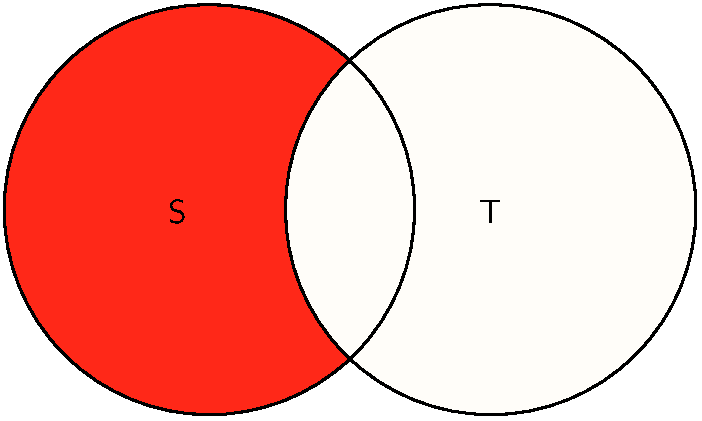
\includegraphics[scale=0.4]{img/difference.pdf}
		\end{figure}
	\end{column}
\end{columns}
\end{frame}

\begin{frame}\frametitle{\insertsection}
	\framesubtitle{\insertsubsection}
   \structure{Beispiel für die Differenzoperation}
\begin{center}
\begin{tabular}{|c|c|c|}\hline
				\multicolumn{2}{|c|}{\footnotesize \textbf{Kunde(S)}}\\\hline\hline
				 \footnotesize \textbf{\key{KNR}} &  \footnotesize \textbf{Nachname}  \\\hline
				\footnotesize 1 &\footnotesize Musterfrau \\\hline
				\footnotesize 2 &\footnotesize  Mustermann  \\\hline
				$\cdots$ &  $\cdots$  \\\hline
			\end{tabular}
			$-$
			\begin{tabular}{|c|c|c|}\hline
				\multicolumn{2}{|c|}{\footnotesize \textbf{Kunde(T)}}\\\hline\hline
				 \footnotesize \textbf{\key{KNR}}  & \footnotesize \textbf{Nachname}  \\\hline
				\footnotesize 1 &\footnotesize Musterfrau \\\hline
				\footnotesize 42 &\footnotesize  Meiser  \\\hline
				$\cdots$ & $\cdots$  \\\hline
			\end{tabular}
			$=$
			\begin{tabular}{|c|c|c|}\hline
				\multicolumn{2}{|c|}{\footnotesize \textbf{Kunde(R)}}\\\hline\hline
				 \footnotesize \textbf{{KNR}} & \footnotesize \textbf{Nachname}  \\\hline
				\footnotesize 2 & \footnotesize  Mustermann  \\\hline
				$\cdots$ & $\cdots$  \\\hline
			\end{tabular}
		\end{center}
\end{frame}

\begin{frame}\frametitle{\insertsection}
\framesubtitle{\insertsubsection}
\onslide
\structure{\textbf{Abgeleitete Operation: Schnitt $\cap$}}
\vspace{5mm}
\begin{columns}
	\begin{column}{.58\textwidth}
		Der Schnitt zweier Relationen $S$ und $T$ aus der gleichen Relationenklasse $\mcl{P}(\mcl{R})$
		besteht aus allen Tupeln, die in $S$ und in $T$ vorkommen.
		\begin{equation*}
		S\cap T=\{r|r\in S \text{\ und\ } r \in T\}
		\end{equation*}
	\end{column}
	\begin{column}{.33\textwidth}
		\begin{figure}
			\vspace{-0.5cm}
			\includegraphics[scale=0.4]{img/intersect.pdf}
		\end{figure}
	\end{column}
\end{columns}
\pause
\abs\abs\abs\abs
Die Schnittoperation leitet sich aus der Differenzoperation ab: $S\cap T = S-(S-T)$.\\
\end{frame}

\begin{frame}\frametitle{\insertsection}
\framesubtitle{\insertsubsection}
\structure{Beispiel für die Schnittoperation}
\begin{center}
\begin{tabular}{|c|c|c|}\hline
				\multicolumn{2}{|c|}{\footnotesize \textbf{Kunde(S)}}\\\hline\hline
				 \footnotesize \textbf{\key{KNR}} &  \footnotesize \textbf{Nachname}  \\\hline
				\footnotesize 1 &\footnotesize Musterfrau \\\hline
				\footnotesize 2 &\footnotesize  Mustermann  \\\hline
				$\cdots$ &  $\cdots$  \\\hline
			\end{tabular}
			$\cap$
			\begin{tabular}{|c|c|c|}\hline
				\multicolumn{2}{|c|}{\footnotesize \textbf{Kunde(T)}}\\\hline\hline
				 \footnotesize \textbf{\key{KNR}}  & \footnotesize \textbf{Nachname}  \\\hline
				\footnotesize 1 &\footnotesize Musterfrau \\\hline
				\footnotesize 42 &\footnotesize  Meiser  \\\hline
				$\cdots$ & $\cdots$  \\\hline
			\end{tabular}
			$=$
			\begin{tabular}{|c|c|c|}\hline
				\multicolumn{2}{|c|}{\footnotesize \textbf{Kunde(R)}}\\\hline\hline
				 \footnotesize \textbf{{KNR}} & \footnotesize \textbf{Nachname}  \\\hline
				\footnotesize 1 & \footnotesize  Musterfrau  \\\hline
				$\cdots$ & $\cdots$  \\\hline
			\end{tabular}
		\end{center}
\end{frame}

\begin{frame}[label=cartProd]\frametitle{\insertsection}
\framesubtitle{\insertsubsection}
\structure{\textbf{Das kartesische Produkt $\times$}}\\[8pt]
$S$ Relation des Schemas $\mcl{R}_1(N\mid A_1,\ldots , A_n)$\\[4pt]
$T$ Relation des Schemas $\mcl{R}_2(N^\prime\mid B_1,\ldots , B_m)$\\[8pt]
Dann ist das kartesische Produkt $S\times T$ die Relation
\begin{equation*}
S\times T = \{(s_1,\ldots,s_n,t_1,\ldots,t_m) \mid (s_1,\ldots s_n) \in S \text{ und } (t_1,\ldots,t_m) \in T \}
\end{equation*}
des Schemas $\mcl{R}_3(N N^\prime\mid A_1,\ldots , A_n,B_1,\ldots ,B_m)$.
\end{frame}

\begin{frame}
\frametitle{\insertsection}
\framesubtitle{\insertsubsection}
\onslide 
\structure{\textbf{Kartesische Produkt $\times$}}\\[8pt]
\begin{itemize}
\item In $S\times T$ werden alle Tupel aus $S$ mit allen Tupeln aus $T$ kombiniert (konkateniert).\\[4pt]
\item Das Ergebnis besteht daher aus $\vert S\vert\cdot\vert T\vert$ Tupeln.\\[8pt]
\pause
\item Ambivalenz:
\begin{itemize}
	\item Falls $\mcl{R}_1$ und $\mcl{R}_2$ gleichnamiges Attribut $A$ haben:\\
	Identifikation bspwse.~durch Relationennamen $N$ und $N^\prime$ {gem\"a\ss} $N.A$ bzw.~$N^\prime.A$\\[8pt]
	\item Dazu sp\"ater mehr.
\end{itemize}
\end{itemize}
\end{frame}

\begin{frame}\frametitle{\insertsection}
\framesubtitle{\insertsubsection}
\structure{Verknüpfung zweier Relationen mit dem kartesischen Produkt}\\[8pt]
Ausgangstabellen:
\begin{columns}
	\begin{column}{.35\textwidth}
		\begin{center}
			\begin{tabular}{|c|c|c|}\hline
				\multicolumn{3}{|c|}{\footnotesize \textbf{Kunde}}\\\hline\hline
				\footnotesize \textbf{\key{KNR}} & \footnotesize \textbf{Vorname} & \footnotesize \textbf{Nachname}  \\\hline
				\footnotesize 1 &\footnotesize Elsa &\footnotesize Musterfrau \\\hline
				\footnotesize 2 & \footnotesize Max &\footnotesize  Mustermann  \\\hline
			\end{tabular}
		\end{center}
	\end{column}
	$\times\quad$
	\begin{column}{.35\textwidth}
		\begin{center}
			\begin{tabular}{|c|c|}\hline
				\multicolumn{2}{|c|}{\footnotesize \textbf{Auftrag}}\\\hline\hline
				\footnotesize \textbf{\key{ANR}} & \footnotesize \textbf{Datum}  \\\hline
				\footnotesize 1001 &\footnotesize 02.01.2013 \\\hline
				\footnotesize 1002 &\footnotesize  04.05.2013  \\\hline
			\end{tabular}
		\end{center}
	\end{column}
\end{columns}
%	\vspace{5mm}
%	Die Relationen sollen mittels des kartesischen Produktes miteinander verknüpft werden.
%	\alert{Achtung: Die Relationenschemata müssen paarweise disjunkt sein, es dürfen daher keine gleichnamigen Attribute existieren!
%	Ergebnis: Siehe Folie \ref{frame:kartesischesProduktErgebnis}.}
\end{frame}

\begin{frame}\label{frame:kartesischesProduktErgebnis}
\frametitle{\insertsection}
\framesubtitle{\insertsubsection}
\structure{Verknüpfung zweier Relationen mit dem kartesischen Produkt}\\[8pt]
	Ergebnisrelation:
	\begin{center}
		\begin{tabular}{|c|c|c|c|c|}\hline
			\multicolumn{5}{|c|}{\footnotesize \textbf{Kunde $\times$ Auftrag}}\\\hline\hline
			\footnotesize{\textbf{KNR}} & \footnotesize{\textbf{Vorname}} & \footnotesize{\textbf{Nachname}} 
			  &\footnotesize{\textbf{ANR}} & \footnotesize{\textbf{Datum}}\\\hline
			1 & Elsa & Musterfrau & 1001  & 02.01.2013\\\hline
			1 & Elsa & Musterfrau & 1002 & 04.05.2013\\\hline
			2 & Max & Mustermann & 1001  & 02.01.2013\\\hline
			2 & Max & Mustermann & 1002  & 04.05.2013\\\hline
		\end{tabular}
	\end{center}
	Jedem Kunden wird jeder Auftrag zugeordnet, was semantisch keinen Sinn ergibt.\\
	Es werden \textit{unechte Tupel} erzeugt $\rightarrow$ dazu später mehr
\end{frame}

\begin{frame}\frametitle{\insertsection}
\framesubtitle{\insertsubsection}
\onslide
\structure{\textbf{Umbenennung}}\\[8pt]
Problemstellung:
\begin{itemize}
	\item Ambivalenz der Namensgebung von Attributen gleichen Namens im kartesischen Produkt 
	\item Semantische Bedeutung von Daten oft mit dem Attributnamen assoziiert
	\item Namen k\"onnen aber obsolet werden\\[8pt]
\end{itemize}
\pause
Ziel:
\begin{itemize}
	\item Operation benötigt, mit deren Hilfe man diesen Umst\"anden Rechnung tragen kann
	\item Datenstruktur des Schemas darf von dieser Operation nicht betroffen sein
\end{itemize}
\end{frame}

\begin{frame}\frametitle{\insertsection}
\framesubtitle{\insertsubsection}
\structure{\textbf{Umbenennung}}\\[8pt]
\begin{block}{}
	Umbenennung von Namen eines Schemas oder von Attributen eines Schemas:
	\begin{itemize}
		\item	Transformation des Schemas $\mcl{R}$ in ein Schema $\mcl{R}^\prime$ mit gleicher Datenstruktur
		\item Erzeugt aus einer Relation $S$ von $\mcl{R}$ eine Relation $S^\prime$ von $\mcl{R}^\prime$
	\end{itemize}
\end{block}
\end{frame}

\begin{frame}\frametitle{\insertsection}
\framesubtitle{\insertsubsection}
\structure{\textbf{Umbenennungsoperation $\rho$}}\\[8pt]
\begin{block}{}
\begin{itemize}
	\item Umbenennung des Attributnamens $A$ in $B$:
	\begin{equation*}
	\rho_{B\leftarrow A}(S)
	\end{equation*} 		
	f\"uhrt Relation $S$ von $\mcl{R}$ in Relation $S^\prime$ \"uber, die Attributnamen $B$ statt $A$ hat.
	\item Umbenennung des Schemanamens $N$ (von Schema $\mcl{R}$) in $N^\prime$ (von Schema $\mcl{R}^\prime$): 
	\begin{equation*}
	\rho_{N^\prime\leftarrow N}(S)
	\end{equation*} 		
	f\"uhrt Relation $S$ von Schema $\mcl{R}$ in Relation $S^\prime$ von Schema $\mcl{R}^\prime$ \"uber, das Schemanamen 
	$N^\prime$ hat.
\end{itemize}
\end{block}
\end{frame}

\begin{frame}\frametitle{\insertsection}
\framesubtitle{\insertsubsection}
\onslide 
\structure{\textbf{Umbenennungsoperation $\rho$}}\\[8pt]
\structure{Beispiel: Umbenennung Attributname}
\begin{center}
S=
\begin{tabular}{|c|c|}\hline
\multicolumn{2}{|c|}{\footnotesize \textbf{Auftrag}}\\\hline\hline
\footnotesize \textbf{\key{ANR}} & \footnotesize \textbf{Datum}  \\\hline
\footnotesize 1001 &\footnotesize 02.01.2013 \\\hline
\footnotesize 1002 &\footnotesize  04.05.2013  \\\hline
\end{tabular}
\pause 
$\quad\quad\rho_{AnNr\leftarrow ANR}(S) =$
\begin{tabular}{|c|c|}\hline
\multicolumn{2}{|c|}{\footnotesize \textbf{Auftrag}}\\\hline\hline
\footnotesize \textbf{\key{AnNr}} & \footnotesize \textbf{Datum}  \\\hline
\footnotesize 1001 &\footnotesize 02.01.2017 \\\hline
\footnotesize 1002 &\footnotesize  04.05.2017  \\\hline
\end{tabular}
\end{center}
\end{frame}

\begin{frame}\frametitle{\insertsection}
\framesubtitle{\insertsubsection}
\onslide 
\structure{\textbf{Umbenennungsoperation $\rho$}}\\[8pt]
\structure{Beispiel: Umbenennung Schemaname}
\begin{center}
S=
\begin{tabular}{|c|c|}\hline
\multicolumn{2}{|c|}{\footnotesize \textbf{Auftrag}}\\\hline\hline
\footnotesize \textbf{\key{ANR}} & \footnotesize \textbf{Datum}  \\\hline
\footnotesize 1001 &\footnotesize 02.01.2013 \\\hline
\footnotesize 1002 &\footnotesize  04.05.2013  \\\hline
\end{tabular}
\pause
$\quad\quad\rho_{Order\leftarrow Auftrag}(S) =$
\begin{tabular}{|c|c|}\hline
\multicolumn{2}{|c|}{\footnotesize \textbf{Order}}\\\hline\hline
\footnotesize \textbf{\key{ANR}} & \footnotesize \textbf{Datum}  \\\hline
\footnotesize 1001 &\footnotesize 02.01.2017 \\\hline
\footnotesize 1002 &\footnotesize  04.05.2017  \\\hline
\end{tabular}
\end{center}
\end{frame}

\begin{frame}
\frametitle{\insertsection}
\framesubtitle{\insertsubsection}
\onslide
\structure{\textbf{Anwendung Umbenennungsoperation $\rho$: \nl Kartesische Produkte von Relationen mit gleichen Attributnamen}}
\abs
Ausgangstabellen:
\begin{columns}
	\begin{column}{.48\textwidth}
		\begin{center}
			\begin{tabular}{|c|c|c|}\hline
				\multicolumn{3}{|c|}{\footnotesize \textbf{Kunde}}\\\hline\hline
				\footnotesize \textbf{\key{KNR}} & \footnotesize \textbf{Vorname} & \footnotesize \textbf{Nachname}  \\\hline
				\footnotesize 1 &\footnotesize Elsa &\footnotesize Musterfrau \\\hline
				\footnotesize 2 & \footnotesize Max &\footnotesize  Mustermann  \\\hline
			\end{tabular}
		\end{center}
	\end{column}
	\begin{column}{.48\textwidth}
		\begin{center}
			\begin{tabular}{|c|c|c|}\hline
				\multicolumn{3}{|c|}{\footnotesize \textbf{Auftrag}}\\\hline\hline
				\footnotesize \textbf{\key{ANR}} & \footnotesize \textbf{KNR}&\footnotesize \textbf{Datum}  \\\hline
				\footnotesize 1001 &\footnotesize 1 &\footnotesize 02.01.2013 \\\hline
				\footnotesize 1002 & \footnotesize 2& \footnotesize  04.05.2013  \\\hline
			\end{tabular}
		\end{center}
	\end{column}
\end{columns}
\abs
\pause
\begin{itemize}
	\item In beiden Relationen existiert das Attribut \texttt{KNR}
	\item Vor Bildung des kartesischen Produktes: Umbenennung der Attribute
	\item Ergebnis: Siehe n\"achste Folie \ref{frame:kartesischesProduktMitUmbenennungErgebnis}.
\end{itemize}
\end{frame}

\begin{frame}	\label{frame:kartesischesProduktMitUmbenennungErgebnis}
\frametitle{\insertsection}
\framesubtitle{\insertsubsection}
\structure{\textbf{Anwendung der Umbenennungsoperation $\rho$: \nl Kartesische Produkte mit Relationen mit gleichen Attributnamen}}
\abs
Ergebnisrelation:
\begin{center}
\begin{tabular}{|c|c|c|c|c|c|}\hline
	\multicolumn{6}{|c|}{\footnotesize \textbf{Kunde $\times$ Auftrag}}\\\hline\hline
	\cellcolor{Yellow}\footnotesize{\textbf{Kunde.KNR}} & \footnotesize{\textbf{Vorname}} & \footnotesize{\textbf{Nachname}} &\footnotesize{\textbf{ANR}} & \cellcolor{Yellow}\footnotesize{\textbf{Auftrag.KNR}}&\footnotesize{\textbf{Datum}}\\\hline
	1 & Elsa & Musterfrau & 1001  & 1 & 02.01.2013\\\hline
	\cellcolor{Red}1 & Elsa & Musterfrau & 1002 &\cellcolor{Red} 2& 04.05.2013\\\hline
	\cellcolor{Red}2 & Max & Mustermann & 1001  &\cellcolor{Red} 1& 02.01.2013\\\hline
	2 & Max & Mustermann & 1002  & 2& 04.05.2013\\\hline
\end{tabular}
\end{center}
\begin{itemize}
\item Nach wie vor werden \backgroundcolour{red}{unechte Tupel} erzeugt, die semantisch nicht zusammen passen. 
\item Auch hierfür gibt es eine Operation, die diesem Umstand begegnet ...
\end{itemize}
\end{frame}

\begin{frame}
\frametitle{\insertsection}
\framesubtitle{\insertsubsection}
\onslide
\structure{\textbf{Selektion $\sigma$}}\\[8pt]
\begin{block}{}
	Selektion von Tupeln einer Relation $R$, die einen Prädikatsausdruck $\theta$ erfüllen.\\
	Ergebnis der Selektionsoperation ist ein Tupel des gleichen Relationenschemas:
	\begin{equation*}
	\sigma_{\theta}(R)=\{t\in R\mid t \text{ erf\"ullt Bedingung } \theta\}
	\end{equation*}
\end{block}
\pause
\abs
Beispiel: $R=Kunde\times Auftrag$, $\theta = (Kunde.KNR=Auftrag.KNR)$
\begin{center}
	\backgroundcolour{green}{$\sigma_{\theta}(R)$} $=$
	\begin{tabular}{|c|c|c|c|c|c|}\hline
		\multicolumn{6}{|c|}{\footnotesize \textbf{Kunde $\times$ Auftrag}}\\\hline\hline
		\footnotesize{\textbf{Kunde.KNR}} & \footnotesize{\textbf{Vorname}} & \footnotesize{\textbf{Nachname}} &\footnotesize{\textbf{ANR}} & \footnotesize{\textbf{Auftrag.KNR}}&\footnotesize{\textbf{Datum}}\\\hline
		\cellcolor{Green}1 &\cellcolor{Green} Elsa & \cellcolor{Green}Musterfrau &\cellcolor{Green} 1001  &\cellcolor{Green} 1 &\cellcolor{Green} 02.01.2013\\\hline
		1 & Elsa & Musterfrau & 1002 &2& 04.05.2013\\\hline
		2 & Max & Mustermann & 1001  &1& 02.01.2013\\\hline
		\cellcolor{Green}2 &\cellcolor{Green} Max & \cellcolor{Green}Mustermann & \cellcolor{Green}1002  & \cellcolor{Green}2&\cellcolor{Green} 04.05.2013\\\hline
	\end{tabular}
\end{center}
\end{frame}

\begin{frame}\frametitle{\insertsection}
\framesubtitle{\insertsubsection}
\structure{\textbf{Im Beispiel: Kombinierte Anwendung}}
\begin{itemize}
	\item Umbenennung: Gemeinsame Attributnamen von zwei Relationen umbenennen\\[5pt]
	\item Kartesisches Produkt: Zwei Relationen vollst\"andig kombinieren 
	\begin{itemize}
		\item unechte Tupel eingeschlossen\\[5pt]
	\end{itemize}
	\item Selektion: Auswahl von Tupeln, die Bedingung (Prädikat) erfüllen
	\begin{itemize}
		\item Selektion echter Tupel m\"oglich
	\end{itemize}
\end{itemize}
\begin{center}
	$\sigma_{\theta}(R)$ $=$
	\begin{tabular}{|c|c|c|c|c|c|}\hline
		\multicolumn{6}{|c|}{\footnotesize \textbf{Kunde $\times$ Auftrag}}\\\hline\hline
		\footnotesize{\textbf{Kunde.KNR}} & \footnotesize{\textbf{Vorname}} & \footnotesize{\textbf{Nachname}} 
		  &\footnotesize{\textbf{ANR}} & \footnotesize{\textbf{Auftrag.KNR}}&\footnotesize{\textbf{Datum}}\\\hline
		1 &Elsa &Musterfrau &1001  &1 &02.01.2013\\\hline
		2 &Max &Mustermann &1002  &2&04.05.2013\\\hline
	\end{tabular}
\end{center}
\end{frame}

\begin{frame}
\frametitle{\insertsection}
\framesubtitle{\insertsubsection}
\onslide
\structure{\textbf{Projektion $\Pi$}}\\[8pt]
\begin{block}{}
	Projektion aller Tupel einer Relation $S$ auf die Attribute einer Attributliste $\{A_1,\dots A_m\}$.\\
	Ergebnis der Projektionsoperation ist eine Relation des projizierten Relationenschemas:
	\begin{equation*}
	\Pi_{\{A_1,\dots A_m\}}(S) = \{\Pi_{\{A_1,\dots A_m\}}(t)\mid t\in S\}
	\end{equation*}
\end{block}
\pause
\abs
Beispiel:
\begin{center}
	$S=$
	\begin{tabular}{|c|c|c|}\hline
		\multicolumn{3}{|c|}{\footnotesize \textbf{Auftrag}}\\\hline\hline
		\footnotesize \textbf{\key{ANR}} & \footnotesize \textbf{KNR}&\footnotesize \textbf{Datum}  \\\hline
		\footnotesize 1001 &\footnotesize 1 &\footnotesize 02.01.2013 \\\hline
		\footnotesize 1002 & \footnotesize 2& \footnotesize  04.05.2013  \\\hline
	\end{tabular}		
	$\quad\Pi_{\{ANR,Datum\}}(S)=$
	\begin{tabular}{|c|c|}\hline
		\multicolumn{2}{|c|}{\footnotesize \textbf{Auftragsdatum}}\\\hline\hline
		\footnotesize \textbf{\key{ANR}} &\footnotesize \textbf{Datum}  \\\hline
		\footnotesize 1001 &\footnotesize 02.01.2013 \\\hline
		\footnotesize 1002 & \footnotesize  04.05.2013  \\\hline
	\end{tabular}
\end{center}
\end{frame}

\begin{frame}\frametitle{\insertsection}
\framesubtitle{\insertsubsection}
\structure{\textbf{Join-Operationen} -- Motivation}\\[8pt]
H\"aufiger Anwendungsfall: 
\begin{itemize}
	\item Kartesisches Produkt einer Relation $S$ eines Prim\"arschemas und einer Relation $R$ eines Fremdschemas
	\item Selektion der Tupel im kartesischen Produkt mit gleichen Werten im Prim\"arschl\"ussel $S.P$ und Fremdschl\"ussel $R.F$
\end{itemize}
\begin{equation*}
\sigma_{(S.P=R.F)}(S\times R)
\end{equation*}
\abs
H\"aufiges Vorkommen dieser Kombination f\"uhrte zur Definition der Join-Operation $\Join$:
\begin{equation*}
S \underset{(S.P = R.F)}{\Join} R := \sigma_{(S.P=R.F)}(S\times R)
\end{equation*}
% 	$$\underset{a \theta b}{S \Join T} \ \mathsf{mit} \ \theta \in \{<,\leq,=,\neq,\geq,>\}, a \in S \wedge b \in T$$
%\vspace{2mm}
%\centerline{$\underset{a \theta b}{S \Join T}$ wird auch $\theta$-Verbund (\textbf{Theta-Join}) genannt}
\end{frame}

\begin{frame}\frametitle{\insertsection}
\framesubtitle{\insertsubsection}
\structure{\textbf{Join-Operationen} -- Motivation}\\[8pt]
Noch einmal das Beispiel:\\ Relationen $Kunde$ und $Auftrag$, Pr\"adikat $\theta = (Kunde.KNR = Auftrag.KNR)$
\begin{center}
	\begin{tabular}{|c|c|c|}\hline
		\multicolumn{3}{|c|}{\footnotesize \textbf{Kunde}}\\ \hline\hline
		\footnotesize \textbf{\key{KNR}} & \footnotesize \textbf{Vorname} & \footnotesize \textbf{Nachname}  \\ \hline
		\footnotesize 1 &\footnotesize Elsa &\footnotesize Musterfrau \\ \hline
		\footnotesize 2 & \footnotesize Max &\footnotesize  Mustermann  \\ \hline
	\end{tabular}
	\hspace{10mm}
	\begin{tabular}{|c|c|c|}\hline
		\multicolumn{3}{|c|}{\footnotesize \textbf{Auftrag}}\\ \hline\hline
		\footnotesize \textbf{\key{ANR}} & \footnotesize \textbf{KNR}&\footnotesize \textbf{Datum}  \\ \hline
		\footnotesize 1001 &\footnotesize 1 &\footnotesize 02.01.2013 \\ \hline
		\footnotesize 1002 & \footnotesize 2& \footnotesize  04.05.2013  \\ \hline
	\end{tabular}
	\abs\abs
	\begin{tabular}{|c|c|c|c|c|c|}\hline
		\multicolumn{6}{|c|}{\footnotesize{ \textbf{Kunde} $\underset{\theta}{\Join}$ \textbf{Auftrag}}}\\\hline\hline
		\footnotesize{\textbf{Kunde.KNR}} & \footnotesize{\textbf{Vorname}} & 
		\footnotesize{\textbf{Nachname}} &\footnotesize{\textbf{ANR}} & 
		\footnotesize{\textbf{Auftrag.KNR}}&\footnotesize{\textbf{Datum}}\\\hline
		1 &Elsa &Musterfrau &1001  &1 &02.01.2013\\\hline
		2 &Max &Mustermann &1002  &2&04.05.2013\\\hline
	\end{tabular}
\end{center}
\end{frame}

\begin{frame}\frametitle{\insertsection}
\framesubtitle{\insertsubsection}
\structure{\textbf{Allgemeine Join-Operationen}}\\[8pt]
\begin{itemize}
	\item Join-Operation nicht nur f\"ur Prim\"ar- und Fremdschl\"usslekombinationen
	\item Join-Operation nicht nur f\"ur Selektion von Tupeln mit gleichen Werten
\end{itemize}
\abs
\textbf{Definition Join-Operation}
\abs
Join-Operation auf Relationen $S$ und $T$ mit beliebigem Selektionspr\"adikat $\theta$:
\begin{equation*}
S \underset{\theta}{\Join} T := \sigma_{\theta}(S\times R)
\end{equation*}
Join-Operation setzt sich aus den elementaren Operationen $\sigma_\theta$ und $\times$ zusammen.
\end{frame}

\begin{frame}\frametitle{\insertsection}
\framesubtitle{\insertsubsection}
\structure{\textbf{Allgemeine Join-Operationen}}\\[8pt]
\begin{alertblock}{Beispiel / \"Ubung}
	\begin{itemize}
		\item Relation $R$ mit Attributen $A_1, A_2,\ldots , A_n$
		\item Relation $S$ mit Attributen $B_1, B_2,\ldots , B_m$
		\item Attribute $A_1$, $A_2$, $A_3$, $B_1$, $B_2$, $B_5$ vom Typ \texttt{integer}
		\item Pr\"adikat $\theta = (A_1 < B_1 \le A_2) \wedge (A_2=B_2) \wedge (A_3 < \frac{1}{2} B_5)$
	\end{itemize}
	\abs
	Beschreiben Sie die Relation $R\underset{\theta}{\Join} S$
\end{alertblock}
\end{frame}

\begin{frame}
\frametitle{\insertsection}
\framesubtitle{\insertsubsection}
\onslide
\structure{\textbf{Equi Join und Natural Join}}\\[8pt]
Besteht $\theta$ eines Join $S \underset{\theta}{\Join} T$
nur aus Gleichheitsaussagen (z.~B.~$\theta = (S.A=T.B) \wedge (S.C=T.D)$), so wird der Join auch 
\textbf{Equi Join} genannt.
\pause
\abs\abs
Werden bei einem Equi Join $S \underset{\theta}{\Join} T$
\begin{itemize}
	\item alle gleichnamigen Attributpaare verkn\"upft 
	\item und in diesem Schema ein Attribut je Attributpaar entfernt,
\end{itemize}
dann nennt man dieses neue Relationenschema \textbf{Natural Join}. Schreibweise: $S \Join T$
\end{frame}

\begin{frame}\frametitle{\insertsection}
\framesubtitle{\insertsubsection}
\structure{\textbf{Equi Join und Natural Join}}\\[8pt]
\begin{alertblock}{Beispiel / \"Ubung}
	\begin{itemize}
		\item Wie sieht ein Equi Join von zwei Relationen aus, die keine paarweise gleichnamigen Attribute haben?\\[6pt]
    %	Existieren keine gleichnamigen Attribute, ist der Natural Join das kartesische Produkt
		\item Beschreiben Sie den Natural Join $S \Join T$ der Relationen $S$ und $T$ mit Attributen $\{A_1,\ldots,A_n,B_1,\ldots, B_m\}$ 
		bzw.~$\{B_1,\ldots, B_m, C_1,\ldots, C_s\}$
		\begin{enumerate}
			\item {\normalsize exemplarisch}\\[4pt]
			\item {\normalsize formal}
		\end{enumerate} 
	\end{itemize}
\end{alertblock}
\end{frame}

\begin{frame}
\frametitle{\insertsection}
\framesubtitle{\insertsubsection}
\onslide
\structure{\textbf{Outer-Join-Operationen}}\\[8pt]
Bisherige Join-Operationen haben nur diejenigen Tupel in die Ergebnisrelation \"uberf\"uhrt, die
\begin{enumerate}
	\item einen entsprechenden Verbundpartner (Tupel) in der anderen Relation haben
	\item die Verbundbedingung $\theta$ erf\"ullt haben
\end{enumerate}
\abs
\pause
Join-Operationen \textbf{Left Outer}, \textbf{Right Outer}, \textbf{Full Outer} enthalten auch Tupel 
\emph{ohne} Verbundpartner:
\begin{itemize}
	\item Left Outer Join $\underset{\theta}\leftouterjoin$ überf\"uhrt \textbf{alle} Tupel der Relation auf der linken Seite des 
	Operators in die Ergebnismenge 
	\item Right Outer Join $\underset{\theta}\rightouterjoin$ überf\"uhrt \textbf{alle} Tupel der Relation auf der rechten Seite 
	des Operators in die Ergebnismenge 
	\item Full Outer Join $\underset{\theta}\fullouterjoin$ ist die Vereinigung von Left und Right Outer Join
\end{itemize}
\end{frame}

\begin{frame}\frametitle{\insertsection}
\framesubtitle{\insertsubsection}
\structure{\textbf{Outer-Join-Operationen} -- Beispiel f\"ur Left Outer Natural Join $\leftouterjoin$}
\begin{center}
	\begin{tabular}{|c|c|c|}\hline
		\multicolumn{3}{|c|}{\footnotesize \textbf{Kunde}}\\\hline\hline
		\footnotesize \textbf{\key{KNR}} & \footnotesize \textbf{Vorname} & \footnotesize \textbf{Nachname}  \\\hline
		\footnotesize 1 &\footnotesize Elsa &\footnotesize Musterfrau \\\hline
		\footnotesize 2 & \footnotesize Max &\footnotesize  Mustermann  \\\hline
		\cellcolor{Yellow}\footnotesize 3 & \cellcolor{Yellow}\footnotesize Hans &\cellcolor{Yellow}\footnotesize Schneider \\\hline
	\end{tabular}
	\hspace{10mm}
	\begin{tabular}{|c|c|c|}\hline
		\multicolumn{3}{|c|}{\footnotesize \textbf{Auftrag}}\\\hline\hline
		\footnotesize \textbf{\key{ANR}} & \footnotesize \textbf{KNR}&\footnotesize \textbf{Datum}  \\\hline
		\footnotesize 1001 &\footnotesize 1 &\footnotesize 02.01.2013 \\\hline
		\footnotesize 1002 & \footnotesize 2& \footnotesize  04.05.2013  \\\hline
	\end{tabular}
	\abs\abs
	\begin{tabular}{|c|c|c|c|c|c|}\hline
		\multicolumn{6}{|c|}{\footnotesize \textbf{Kunde} $\leftouterjoin$ \textbf{Auftrag}}\\\hline\hline
		\footnotesize{\textbf{Kunde.KNR}} & \footnotesize{\textbf{Vorname}} & 
		\footnotesize{\textbf{Nachname}} &\footnotesize{\textbf{ANR}} & 
		\footnotesize{\textbf{Auftrag.KNR}}&\footnotesize{\textbf{Datum}}\\\hline
		\footnotesize 1 & \footnotesize Elsa & \footnotesize Musterfrau &\footnotesize 1001  &\footnotesize 1 &\footnotesize 02.01.2013\\\hline
		\footnotesize 2 & \footnotesize & \footnotesize Mustermann &\footnotesize 1002  &\footnotesize 2& 04.05.2013\\\hline
		\cellcolor{Yellow}\footnotesize 3 &\cellcolor{Yellow}\footnotesize Hans&\cellcolor{Yellow}\footnotesize Schneider
		&\cellcolor{Yellow}\footnotesize\texttt{null}&\cellcolor{Yellow}\footnotesize\texttt{null}
		&\cellcolor{Yellow}\footnotesize\texttt{null}\\\hline
	\end{tabular}
\end{center}
\end{frame}

\begin{frame}
\frametitle{\insertsection}
\framesubtitle{\insertsubsection}
\structure{\textbf{Outer-Join-Operationen}}\\[8pt]
Outer Join-Operationen lassen sich auf die elementaren Operationen 
$\sigma_\theta$, $\times$, $\cup$, $-$, $\Pi$ der relationalen Algebra zur\"uckf\"uhren:
\abs
\begin{theorem}
	\begin{equation*}
	\begin{split}
	R\underset{\theta}\leftouterjoin S &= (R\underset{\theta}\Join S) \cup (R - \Pi_{Attr(R)}(R\Join S)) \times 
	\{\texttt{null},\ldots ,\texttt{null}\}\\
	R\underset{\theta}\rightouterjoin S &= (R\underset{\theta}\Join S)\cup \{\texttt{null},\ldots ,\texttt{null}\}\times 
	(S - \Pi_{Attr(S)}(R\Join S))\\
	R\underset{\theta}\fullouterjoin S &= R\underset{\theta}\leftouterjoin S\cup R\underset{\theta}\rightouterjoin S
	\end{split} 
	\end{equation*}
\end{theorem}
\abs
Beachte: Join-Operation $\underset{\theta}\Join$ setzt sich aus elementaren Operationen $\sigma_\theta$ und $\times$ zusammen.
\end{frame}

\begin{frame}
\frametitle{\insertsection}
\framesubtitle{\insertsubsection}
\structure{\textbf{Aggregation}}\\[8pt]
\begin{itemize}
	\item Aggregation ist ein Operationstyp auf Relationen, 
	der nicht durch die elementaren Operationen der relationalen Algebra ausgedr\"uckt werden kann.
	\item Aggregationen sind somit \textit{nicht} Bestandteil der klassischen relationalen Algebra
	\item Sie wurden als Erweiterung eingef\"uhrt.
	\item Aggregatsfunktionen berechnen aus mehreren (m\"oglicherweise gleichen) Werten einen neuen Wert, das sogenannte Aggregat.
	Beispiele: 
	\begin{itemize}
		\item Summe
		\item Durchschnitt
		\item Minimum oder Maximum
		\item Anzahl
	\end{itemize}
\end{itemize}
\end{frame}

\begin{frame}
\frametitle{\insertsection}
\framesubtitle{\insertsubsection}
\onslide 
\structure{\textbf{Aggregation} -- Motivation}\\[-12pt]
\begin{columns}
	\begin{column}{.3\textwidth}		
		\begin{figure} 
			\includegraphics[scale=0.45]{img/Table_Aggregate_raw.png}\\[-9pt]
			{\tiny Mitarbeiterdaten}
		\end{figure}
	\end{column}
	\pause
	\begin{column}{.3\textwidth}		
		\begin{figure} 
			\includegraphics[scale=0.45]{img/Table_Aggregate_group.png}\\[-9pt]
			{\tiny Mitarbeiter gruppiert nach (Status, Abteilung)}
		\end{figure}
	\end{column}
\end{columns}
\pause 
\begin{figure} 
	\includegraphics[scale=0.45]{img/Table_Aggregate_aggr.png}\\[-8pt]
	{\tiny Mitarbeiterdaten aggregiert nach Gruppen}
\end{figure}
\end{frame}

\begin{frame}
\frametitle{\insertsection}
\framesubtitle{\insertsubsection}
\onslide
\structure{\textbf{Aggregation}}\\[3pt]
\begin{itemize}
	\item $R$ Relation des Schemas $\mcl{R}(G_1,\ldots , G_n, A_1, \ldots , A_m,B_1,\ldots , B_p)$.
	\item Schema $\mcl{R}$ hat Gruppierungsattribute $\{G_1,\ldots , G_n\}$ und Aggregationssattribute $\{A_1,\ldots , A_m\}$
	\begin{itemize}
		\item Im Beispiel: $G_1=\texttt{Status}$, $G_2=\texttt{Abteilung}$, $A_1=\texttt{Gehalt}$, $A_2=\texttt{Jahre}$
	\end{itemize}
	\pause
	\item Datens\"atze in Relation $R$ werden gruppiert nach den unterschiedlichen Werten $(g_1, \ldots , g_n)$ in den Attributen 
	$\{G_1,\ldots , G_n\}$.
	\pause
	\item In jeder dieser Gruppen werden Aggregate aus den Werten der einzelnen Aggregationssattribute $\{A_1,\ldots , A_m\}$
	ermittelt.
	\pause
	\item Neue Tabelle $S$ mit folgenden Spalten: $G_1,\ldots , G_n$, Spalte je Aggregatstyp
	\begin{itemize}
		\item Im Beispiel:
		\nl $G_1=\texttt{Status}$, $G_2=\texttt{Abteilung}$; 
		\nl $\texttt{AVG(Gehalt)}$, $\texttt{MIN(Gehalt)}$, $\texttt{AVG(Jahre)}$ 
	\end{itemize} 
	\pause
	\item Bezeichnung: 
	$S= \Gamma_{\texttt{Status,}\,\texttt{Abteilung\,;}\,
		\texttt{AVG(Gehalt),}\,\texttt{MIN(Gehalt),}\,\texttt{AVG(Jahre)}}(R)$
\end{itemize} 	
\end{frame}

% vvvvvv weglassen vvvvvv
\nowrite{ 
\begin{frame}
\frametitle{\insertsection}
\framesubtitle{\insertsubsection}
\structure{\textbf{Aggregation} -- Notation und formale Beschreibung}\\[3pt]
\begin{itemize}
	\item $R$ Relation des Schemas $\mcl{R}(G_1,\ldots , G_n, A_1, \ldots , A_m,B_1,\ldots , B_p)$.
	\item $R$ partitioniert in (disjunkte) Gruppen $G_{(g_1, \ldots , g_n)}$
	mit Werten $(g_1, \ldots , g_n)$ in den Attributen $(G_1, \ldots , G_n)$.
	\item F\"ur jede Gruppe $G_{(g_1, \ldots , g_n)}\subseteq R$ und zu jedem Attribut $A_i$ ist $ M_{i,(g_1, \ldots , g_n)}$ die Multi-Menge 
	\begin{equation*}
	M_{i,(g_1, \ldots , g_n)} = [x\mid x=\Pi_{A_i}(r) \text{ f\"ur } r \in G_{(g_1, \ldots , g_n)}]
	\end{equation*}
	\item F\"ur jedes aggregierbare Attribut $A_i$ gibt es Aggregationsfunktionen $F^1_i, F^2_i, \ldots , F^{q_i}_i$.
	\item F\"ur jede Gruppe $G_{(g_1, \ldots , g_n)}\subseteq R$ und zu jedem Attribut $A_i$ bilde die Werte 
	\begin{equation*}
	f^1_{i,(g_1, \ldots , g_n)} = F^1_i(M_{i,(g_1, \ldots , g_n)}), \ldots , 
	f^{q_i}_{i,(g_1, \ldots , g_n)} =F^{q_i}_i(M_{i,(g_1, \ldots , g_n)})    
	\end{equation*}
\end{itemize}
\end{frame}
%
\begin{frame}
\frametitle{\insertsection}
\framesubtitle{\insertsubsection}
\structure{\textbf{Aggregation} -- Definition}\\[3pt]
\begin{itemize}
\item $R$ Relation des Schemas $\mcl{R}(G_1,\ldots , G_n, A_1, \ldots , A_m,B_1,\ldots , B_p)$.
%\item Gruppierungsschema: $\mcl{S}(G_1,\ldots , G_n, F^1_1(A_1), \ldots , F^{q_m}_m(A_m))$ 
\item Relation $S$ ist definiert durch % $S$ im Schema $\mcl{S}$
\begin{equation*}
\begin{split}
S=\{t\mid &t=(g_1, \ldots , g_n, f^1_{1,(g_1, \ldots , g_n)}, \ldots f^{q_m}_{m,(g_1, \ldots , g_n)}) \text{ mit }\\
&(g_1, \ldots , g_n) =\Pi_{(G_1,\ldots , G_n)}(r) \text{ f\"ur } r\in R\}
\end{split}
\end{equation*}
\item Relation $S$ ist die \textbf{Aggregation} von $R$ auf den Attributen $A_1, \ldots , A_m$
entlang der Gruppierung $(G_1, \ldots , G_n)$.
\begin{equation*}
\text{Bezeichnung:}\quad\quad\quad\quad\quad\quad S= \Gamma_{G_1, \ldots , G_n; F^1_1(A_1), \ldots , F^{q_m}_m(A_m)}(R)
\phantom{xxxxxxxxxxxxxxxxxxxxxxxxxxxxxxxxxxxxxxxxxx}
\end{equation*}
\end{itemize}
\end{frame}
}
% ^^^^^^ weglassen ^^^^^^

\begin{frame}
\frametitle{\insertsection}
\framesubtitle{\insertsubsection}
\onslide 
\structure{\textbf{Aggregation} -- noch einmal zur\"uck zum Beispiel}
\begin{columns}
	\begin{column}{.3\textwidth}		
		\begin{figure} 
			\includegraphics[scale=0.45]{img/Table_Aggregate_raw.png}\\[-9pt]
			{\tiny Relation Mitarbeiter}
		\end{figure}
	\end{column}
	\pause
	\begin{column}{.6\textwidth}		
		\begin{figure} 
			\includegraphics[scale=0.45]{img/Table_Aggregate_aggr.png}\\[-8pt]
			{\tiny Mitarbeiterdaten aggregiert nach Gruppen}
		\end{figure}
	\end{column}
\end{columns}
\abs\abs
\centering Aggregation: $\Gamma_{\texttt{Status,}\,\texttt{Abteilung\,;}\,
	\texttt{AVG(Gehalt),}\,\texttt{MIN(Gehalt),}\,\texttt{AVG(Jahre)}}(R)$
\end{frame}

% vvvvvv weglassen vvvvvv
\nowrite{ 
\begin{frame}
\frametitle{\insertsection}
\framesubtitle{\insertsubsection}
\structure{Bildung von Aggregaten}
Beispiel: $\Gamma_{KNR, count(*), sum(Wert)}(Auftrag)$
\begin{center}
	\footnotesize
	\begin{tabular}{|c|c|c|}\hline
		\multicolumn{3}{|c|}{\footnotesize \textbf{Auftrag}}\\\hline\hline
		\footnotesize \textbf{\key{ANR}} & \footnotesize{\textbf{KNR}} & \footnotesize \textbf{Wert}  \\\hline
		\footnotesize 1001 & 1 &\footnotesize 10,12 \\\hline
		\footnotesize 1002 & 2 & \footnotesize  12,13  \\\hline
		\footnotesize 1003 & 1 & \footnotesize  14,23  \\\hline
	\end{tabular}
	\hspace{3em}
		\begin{tabular}{|c|c|c|}\hline
			\multicolumn{3}{|c|}{\footnotesize \textbf{$\Gamma_{KNR, count(*), sum(Wert)}(Auftrag)$}}\\\hline\hline
			\footnotesize \textbf{\textbf{KNR}} & \footnotesize{\textbf{count(*)}} & \footnotesize \textbf{sum(Wert)}  \\\hline
			\footnotesize 1 & 2 &\footnotesize 24,35 \\\hline
			\footnotesize 2 & 1 & \footnotesize  12,13  \\\hline
		\end{tabular}
\end{center}
\alert{Nicht-aggregierte Attribute werden als Gruppierungsattribute herangezogen!}
\end{frame}
}
% ^^^^^^ weglassen ^^^^^^

\section*{Übungsaufgaben}
\begin{frame}[t]
	\frametitle{\insertsection}	
	\begin{alertblock}{Relationenmodell und relationale Algebra}
		\begin{enumerate}
			\item Erläutern Sie die Begriffe \emph{Relationenschema} und \emph{Relation eines Relationenschemas}.
			\item Grenzen Sie die Begriffe \textit{funktional abhängig} und \textit{voll funktional abhängig} voneinander ab.
			\item Erläutern Sie den Zusammenhang zwischen funktionaler Abhängigkeit und dem Konzept eines \textit{Schlüssels}.
			\item Für die Identifikation eines Tupels kann jeder Kandidatenschlüssel als Primärschlüssel ausgewählt werden. 
			In welche Situationen könnte einem Kandidatenschlüssel $K_1$ gegenüber einem Kandidatenschlüssel $K_2$ der Vorzug gegeben werden?
			\item Warum ist die Operation $\rho$ essentiell in der relationalen Algebra?
			\item Beschreiben Sie den $\theta$-Join durch elementare Operationen der relationalen Algebra.
			\item Was unterscheidet den Aggregations-Operator $\Gamma$ von den übrigen Operationen der relationalen Algebra?
		\end{enumerate}
	\end{alertblock}
\end{frame}
